\documentclass[a4paper, 11pt]{article}
\pdfoutput=1 % if your are submitting a pdflatex (i.e. if you have
             % images in pdf, png or jpg format)

\usepackage{jcappub} % for details on the use of the package, please
                     % see the JCAP-author-manual

\usepackage[T1]{fontenc} % if needed

\usepackage{array}
\usepackage{enumitem}
\usepackage{graphicx}
\usepackage{epstopdf, epsfig}
\usepackage{subcaption}
\usepackage{tikz}
\usetikzlibrary{intersections}
\usepackage{pgfplots}
\usepackage{ environ}
\usepackage{framed}
\usepackage{bm}
\usepackage[us,12hr]{datetime}
\usepackage{algorithmic}
\usepackage[ruled]{algorithm2e}

\title{2D Caustic Skeleton II: Constraint Realization of the Cosmic Web}

\author[a,b]{Job Feldbrugge}
\author[c]{Rien van de Weygaert}

\affiliation[a]{Higgs Centre for Theoretical Physics, University of Edinburgh, Edinburgh, Scotland, EH8 9YL}
\affiliation[b]{Physics department, Carnegie Mellon University, Pittsburgh, United States}
\affiliation[c]{Kapteyn Astronomical Institute, University of Groningen, Groningen, The Netherlands}

\emailAdd{jfeldbrugge@perimeterinstitute.ca}

\newcommand{\aap}{Astron. Astrophys.}
\newcommand{\mnras}{Mon. Not. R. Astron. Soc.}
\newcommand{\apj}{Astrophys. J.}
\newcommand{\jcap}{Journal of Cosmology and Astroparticle Physics}
\newcommand{\nat}{Nature}
\newcommand{\apjs}{Astrophysical Journal, Supplement}
\newcommand{\apjl}{Astrophysical Journal, Letters}
\newcommand{\aj}{Astronomical Journal}
\newcommand{\prd}{Physical Review D}

\newcommand{\Remark}[1]      {{\small {\textcolor{red}{  \sf{[[{#1}]]}}}}} 

\newtheorem{thr}{Theorem:}
\newtheorem{lemma}{Lemma}
\newtheorem{corollary}{Corollary}

\abstract{
\noindent Last compiled on: {\color{red} \currenttime\ at \today}}

\graphicspath{
{./figures/}}

\begin{document}
%\pagecolor{yellow!30!orange}
\maketitle



\newpage
%%%%%%%%%%%%%%%%%%%%%%%%%%%%%%%%%%%%%%%%%%%%%%%%%%%%%%%%%%%%%%%%
\section{Introduction}
The large-scale structure of our Universe -- consisting of large voids, thin membranes, thick filaments, and massive clusters -- are now routinely observed through the distribution of galaxies, neutral gas, and dark matter. Upcoming cosmological redshift surveys will map the \textit{cosmic web} in even greater detail, revealing a lot of information about its geometry and topology, the properties of the embedded galaxies, and fundamental physics. Remarkably, the cosmic web is not only observable through the distribution of galaxies, but, in fact, directly influences their formation processes. Cosmic streams flow along the filamentary structure of the cosmic web influencing the angular momentum and spin alignment of the embedded galaxies. Given the detail of the next generation of cosmological surveys, it is increasingly important to develop an analytic framework that models the mildly non-linear evolution of the different features of the cosmic web -- the voids, the walls, the filaments and the clusters -- and their influence on the embedded halos and galaxies.

Building on work by Arnol'd, Zel'dovich and collaborators, we recently solved a long-standing problem in Lagrangian catastrophe theory, enabling us to build such a framework. We track the evolution of the dark matter sheet in six-dimensional \textit{phase-space} and mark the locations where the fluid forms caustics, highlighting the place and time where gravitational collapse turns non-linear and walls, filaments, and clusters emerge. Moreover, these caustic mark the locations where these structures merge to form the interconnected structure which we observe today. When combining caustic theory with an analytic model of large-scale structure formation, such as the Zel'dovich approximation, these caustics define the \textit{caustic skeleton}, marking the locations and configurations in the initial conditions that are the progenitors of the intricate geometric cosmic pattern. This approach turns out to be remarkably successful at predicting the cosmic geometry and topology of the cosmic web from the much simpler Gaussian initial conditions.

Over the last decades, there have been many attempts to analyze the relationship between the initial conditions and the emergence of the cosmic web. Consider for example the application of Morse-Smale theory, where the minima, saddle points, and maxima are linked to the voids, membranes, filaments and clusters. Constrained Gaussian random field theory is an ideal tool to study these proposals systematically by generating realistic initial conditions satisfying these linear constraint. By evolving these initial conditions, one can analyze the link between the critical points in the initial density field and the emerging non-linear structure. However, so far constrained Gaussian random field theory has been limited to linear constraints. The specified conditions, moreover only have an intuitive link with the dynamics of gravitational collapse. 

In this paper, we extend constrained Gaussian random field theory to non-linear constraints. We demonstrate how this method can be used to generate initial conditions satisfying the non-linear caustic conditions, tying the constraints to the dynamics of gravitational collapse. By running a set of small N-body simulations, we investigate how the caustic skeleton compares with the non-linear large scale structure and study the characteristic properties of the features of the cosmic web. In this paper, we limit our investigation to the two-dimensional cosmic web consisting of voids, filaments and clusters. However, the techniques straightforwardly extend to the three-dimensional Universe.

















%%%%%%%%%%%%%%%%%%%%%%%%%%%%%%%%%%%%%%%%%%%%%%%%%%%%%%%%%%%%%%%%
\section{Caustic skeleton theory}
 


%%%%%%%%%%%%%%%%%%%%%%%%%%%%%%%%%%%%%%%%%%%%%%%%%%%%%%%%%%%%%%%%
\subsection{Lagrangian fluid dynamics}
Lagrangian fluid dynamics is well-known to be an effective tool to model the cosmic web, as exemplified by the famous Zel'dovich approximation, second-order Lagrangian perturbation theory ($2$LPT), and $N$-body simulations. The Lagrangian fluid consists of a collection of mass elements, evolving according to the Lagrangian map $\bm{x}_t:\mathcal{L}\to \mathcal{E}$,
\begin{align}
\bm{x}_t(\bm{q}) \equiv \bm{q} + \bm{s}_t(\bm{q})\,,
\end{align}
with the displacement field $\bm{s}_t$, describing the motion of the mass elements from the initial position $\bm{q}$ in Lagrangian space $\mathcal{L}$ to the final position $\bm{x}_t(\bm{q})$ at time $t$ in Eulerian space $\mathcal{E}$. A mass element can flow, stretch, and rotate, while conserving its mass. A two-dimensional fluid forms a two-dimensional sheet $M_t=\{(\bm{q},\bm{x}_t(\bm{q})) | \bm{q}\in \mathcal{L}\}$ in four-dimensional \textit{phase-space} $\mathcal{L}\times \mathcal{E}$, consisting of the inital and the final position of the mass element. Note that there exists a direct relation between this phase-space and the more conventional phase-space consisting of the position and momentum of the particle used in Hamiltonian mechanics. The cosmic web emerges when mapping the dark matter sheet $M_t$ onto the final position $\varphi:\mathcal{L}\times \mathcal{E} \to \mathcal{E}$, defined by $(\bm{q},\bm{x}) \mapsto\bm{x}$ (see figure \ref{fig:Phase-Space} for an illustration).

\begin{figure}
\centering
\begin{subfigure}[b]{0.49\textwidth}
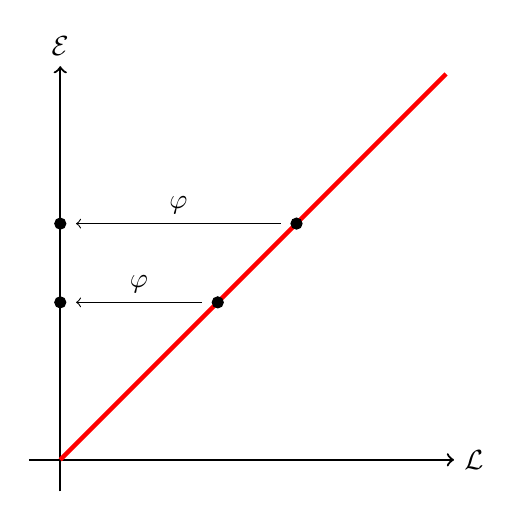
\begin{tikzpicture}
%\draw[help lines, color=gray!30, dashed] (-0.9,-0.9) grid (4.9,4.9);
\draw[->, thick] (-0.4,0)--(5,0) node[right]{$\mathcal{L}$};
\draw[->, thick] (0,-0.4)--(0,5) node[above]{$\mathcal{E}$};
\draw[-,ultra thick, red] (0,0)--(4.9,4.9);
\filldraw[black] (2,2) circle (2pt);
\filldraw[black] (0,2) circle (2pt);
\filldraw[black] (3,3) circle (2pt);
\filldraw[black] (0,3) circle (2pt);
\draw[->] (1.8,2) -- node[above] {$\varphi$} ++ (-1.6,0);
\draw[->] (2.8,3) -- node[above] {$\varphi$} ++ (-2.6,0);
\end{tikzpicture}
\end{subfigure}~
\begin{subfigure}[b]{0.49\textwidth}
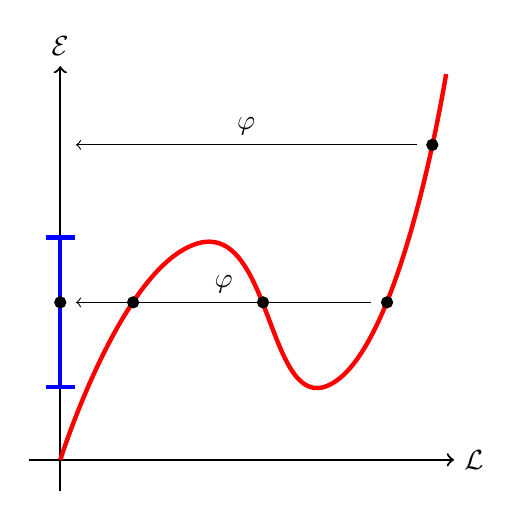
\begin{tikzpicture}
%\draw[help lines, color=gray!30, dashed] (-0.9,-0.9) grid (4.9,4.9);
\draw[->, thick] (-0.4,0)--(5,0) node[right]{$\mathcal{L}$};
\draw[->, thick] (0,-0.4)--(0,5) node[above]{$\mathcal{E}$};
\draw[|-|,ultra thick, blue] (0,0.9)--(0,2.85);
\draw [-, ultra thick, red] plot [smooth, tension=1] coordinates { (0,0) (1.75,2.75)  (3.5,1) (4.9,4.9)};
\filldraw[black] (0,2) circle (2pt);
\filldraw[black] (0.925,2) circle (2pt);
\filldraw[black] (2.575,2) circle (2pt);
\filldraw[black] (4.15,2) circle (2pt);
\filldraw[black] (4.725,4.) circle (2pt);
\draw[->] (3.95,2) -- node[above] {$\varphi$} ++ (-3.75,0);
\draw[->] (4.525,4.) -- node[above] {$\varphi$} ++ (-4.325,0);
\end{tikzpicture}
\end{subfigure}
\caption{Projection of phase-space to Eulerian space. The left panel illustrates the initial dark matter sheet in phase space. The arrow represents the projection to Eulerian space $\varphi$. The mapping is one-to-one. The right panel illustrates the dark matter sheet after it has evolved and formed a triple-stream region (in blue). Each point in the triple-stream region corresponds to three points on the dark matter sheet. The triple-stream region is bounded by a fold caustic at which matter shell crosses.}\label{fig:Phase-Space}
\end{figure}

Initially, the displacement field vanishes, $\bm{s}_0(\bm{q})=\bm{0}$, and the phase-space manifold is diagonal $M_0=\{(\bm{q},\bm{q})|\bm{q} \in \mathcal{L}\}$. The mapping $\varphi$ is one-to-one, corresponding to a single-stream region (see the left panel of figure\ \ref{fig:Phase-Space}). When the fluid evolves, the phase-space manifold can develop complex configurations at which the mapping $\varphi$ becomes many-to-one, \textit{i.e.}, a final position can be reached from multiple initial positions (see the right panel of figure \ref{fig:Phase-Space}). The connected region in Eulerian space with $n$ possible initial positions is known as a $n$-stream region. In these multi-stream regions, gravitational collapse becomes mildly non-linear and viralized structures form. Note that the multi-stream regions uniquely partition the universe based on the dynamics of gravitational collapse. As we will show in the next section, different multi-stream regions can be associated to the membranes, filaments, and clusters of the cosmic web. The single-stream regions correspond to the voids, where the evolution of the cosmic web remains largely linear.

The density of a Lagrangian fluid evolves while the mass elements are squeezed and stretched, \textit{i.e.},
\begin{align}
\rho_t(\bm{x})
&= \sum_{\bm{q} \in A_t(\bm{x})} \frac{\bar{\rho}}{|\det \nabla \bm{x}_t(\bm{q})|}\\
&= \sum_{\bm{q} \in A_t(\bm{x})} \frac{\bar{\rho}}{|1+\mu_{t,1}(\bm{q})||1+\mu_{t,2}(\bm{q})|}\,,
\label{eq:density}
\end{align}
with the mean initial density $\bar{\rho}$, and the eigenvalue fields $\mu_{t,1}$ and $\mu_{t,2}$ of the deformation tensor $\nabla \bm{s}_t$, defined by
\begin{align}
\nabla \bm{s}_t(\bm{q}) \bm{v}_{t,i}(\bm{q}) = \mu_{t,i}(\bm{q}) \bm{v}_{t,i}(\bm{q})\,.
\label{eq:EigenvalueAndEigenvector}
\end{align} 
Each stream contributes to the density, as the sum runs over the points that reach $\bm{x}$ in time $t$, \textit{i.e.},
\begin{align}
A_t(\bm{x}') = \{\bm{q}|\bm{x}_t(\bm{q})=\bm{x}'\}\,.
\end{align}
The boundaries of the multi-stream regions mark discontinuous of the density field \eqref{eq:density}. In fact, in these regions the mass elements flip orientation in a process known as \textit{shell-crossing}, for which the determinant $\det \nabla \bm{x}_t$ vanishes and the density spikes to infinity. This phenomenon is an example of a \textit{fold caustic}, bounding the regions where virialized structures emerge. We always order the eigenvalue fields such that $\mu_{t,1}$ corresponds to the first shell-crossing. In the next section we show that the -- often ignored -- corresponding eigenvector fields $\bm{v}_{t,i}$ play an important role in the higher order caustics structure formation. 

In the current theory of late time cosmology, the cosmic web formed due to the gravitational collapse of tiny Gaussian fluctuations $\delta_0$ (see section \ref{sec:GRF} for a detailed discussion on Gaussian random field theory). At early times, the dynamics of the mass elements was governed by the corresponding initial gravitational potential $\phi_0$ through the displacement field $\bm{s}_t$ which turns out to be propertional to the gradient of the initial gravitational potential (see section \ref{sec:Zeldovich} for a detailed discussion). See the upper panels of figure \ref{fig:Initial_Conditions} for an illustration of a reasonable initial density and the corresponding gravitational potential field. 

Eulerian fluid dynamics describes the evolution of the large scale structure in terms of these Gaussian density and gravitational potential fields. In contract, Lagrangian fluid dynamics emphasises the role of the deformation tensor $\nabla \bm{s}_t$ and the corresponding eigenvalue and eigenvector fields (which is apparent from the density formula \eqref{eq:density}). The defining equation \eqref{eq:EigenvalueAndEigenvector} implies a non-linear relation between the partial derivatives of the displacement field and eigenvalue and eigenvector fields (quadratic in 2D and cubic in 3D). At early times the deformation tensor $\nabla \bm{s}_t$ is proportional to the Hessian of the gravitational potential, $\nabla \bm{s}_t \propto \mathcal{H}\phi_0$, and the eigenvalue and eigenvector fields are expressed as nonlinear functions of the second order derivatives of the initial gravitational potential. It follows that early time Lagrangian fluid dynamics is governed by a non-Gaussian random field, capturing part of the non-linearity of gravitational collapse. See the lower panels of figure \ref{fig:Initial_Conditions} for an illustration of the non-Gaussian eigenvalue  fields, where the red regions experience the strongest gravitational collapse and blue regions represent an outflow of matter. Observe that the eigenvalue fields, roughly speaking, peak in the regions of high initial density. In particular, compare the peaks of the initial density field $\delta_0$ and the second eigenvalue field $\mu_{t,2}$. However, the density perturbation and the eigenvalue fields differ away from the high density regions. The eigenvalue fields emphasise line like features connecting the high density regions. As described below, these line-like features of the first eigenvalue field are progenitors of the filaments of the cosmic web.


\begin{figure}
\centering
\begin{subfigure}[b]{0.49\textwidth}
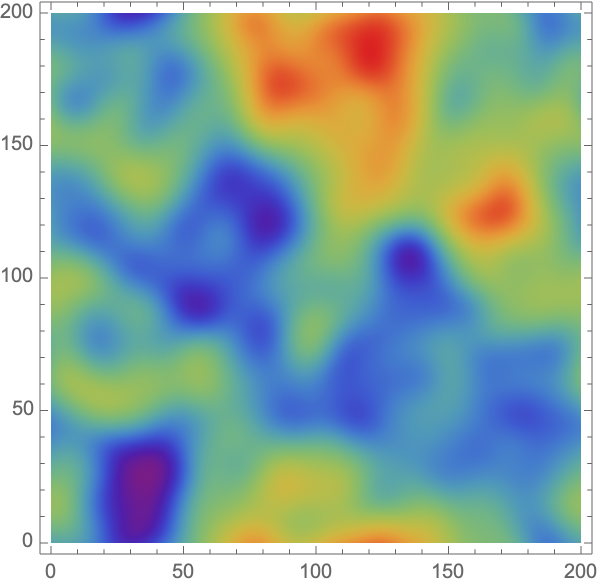
\includegraphics[width=\textwidth]{Psi}
\end{subfigure}~
\begin{subfigure}[b]{0.49\textwidth}
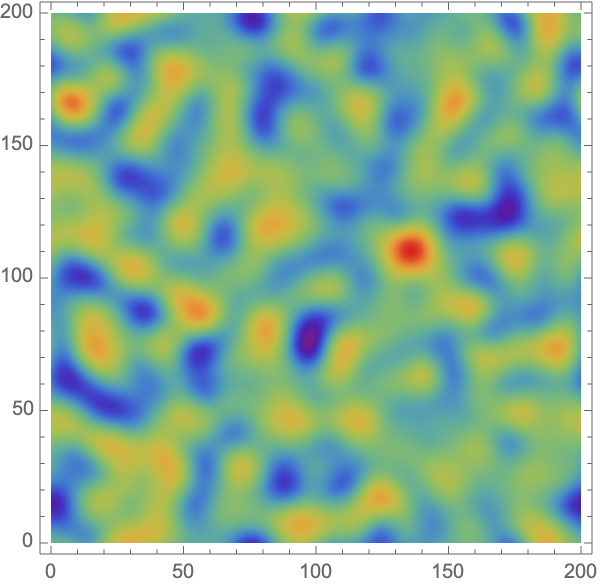
\includegraphics[width=\textwidth]{Rho}
\end{subfigure}\\
\begin{subfigure}[b]{0.49\textwidth}
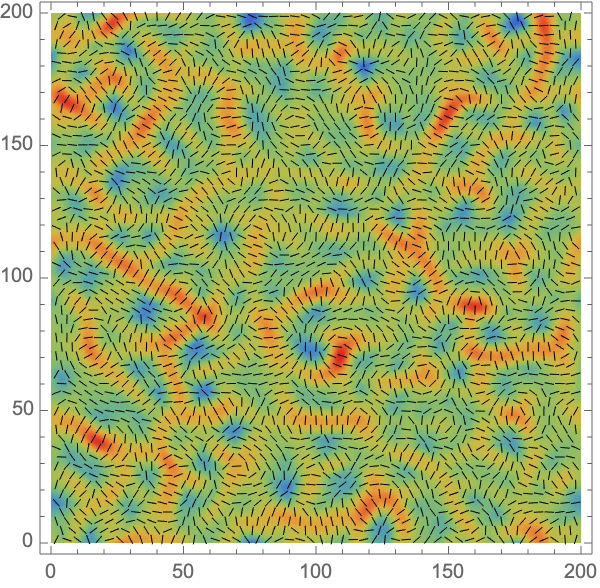
\includegraphics[width=\textwidth]{Lambda_1}
\end{subfigure}~
\begin{subfigure}[b]{0.49\textwidth}
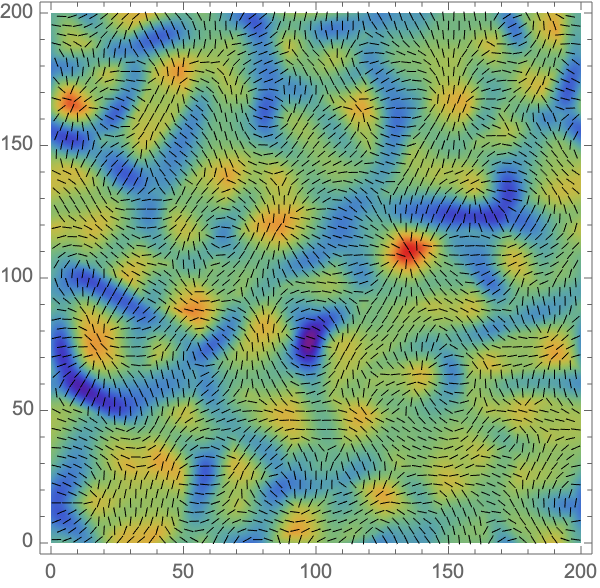
\includegraphics[width=\textwidth]{Lambda_2}
\end{subfigure}
\caption{A Gaussian random field and the corresponding eigenvalue and eigenvector fields. \textit{Upper left:} the gravitaitonal potential $\Psi$. \textit{Upper right:} the corresponding density perturbation field $\delta$. \textit{Lower left:} the first eigenvalue and eigenvector fields $\mu_1,\bm{v}_1$. \textit{Lower right:} the second eigenvalue and eigenvector fields $\mu_2,\bm{v}_2$.}\label{fig:Initial_Conditions}
\end{figure}


It follows from the Poisson equation (see section \ref{sec:Zeldovich}), that the sum of the initial eigenvalue fields is proportional to the initial density perturbation, 
\begin{align}
\delta_0 \propto \nabla^2 \phi_0 = \text{Tr}[\mathcal{H}\phi_0] \propto \mu_{t,1} + \mu_{t,1}\,,
\end{align}
demonstrating a non-trivial correlation between the initial eigenvalue fields. The eigenvalue fields splits the Gaussian initial density perturbations into parts which influence the linear regime of gravitational collapse in distinct ways. As we will show below, the orientation and geometry of the shell-crossing regions is further described by the eigenvector fields (see the lines in the lower panels of figure \ref{fig:Initial_Conditions}). At initial times, the eigenvector fields are normal, $\bm{v}_{t,1}\cdot \bm{v}_{t,2}=0$, as the deformation tensor $\nabla \bm{s}_t \propto \mathcal{H} \phi_0$ is symmetric. We observe that the eigenvector fields show an interesting correlation with the eigenvalue fields. Roughly speaking, the eigenvector fields are normal to the ridges of the corresponding eigenvalue fields. This observation will play an important role in the discussion of the caustic skeleton below. 

%%%%%%%%%%%%%%%%%%%%%%%%%%%%%%%%%%%%%%%%%%%%%%%%%%%%%%%%%%%%%%%%
\subsection{Caustics Lagrangian fluids}
The study of the cosmic web in terms of multi-stream regions and Lagrangian catastrophe theory has a rich history, predating the developments of $N$-body simulations (REFS). Amazingly, by analysing the geometry of the caustics emerging in Lagrangian fluid dynamics, Y.\ Zel'dovich, V.\ Arnol'd and collaborators successfully predicted the qualitative features of the cosmic web. However, these studies where mainly restricted to two-dimensional models, as several technical problems inhibited the full treatment of three-dimensional cosmic web. In a recent publication (REF), we solved these problems by formulating the \textit{shell-crossing condition} describing how a submanifold in $\mathcal{L}$ can develop a non-differentiable feature under the mapping $\bm{x}_t$. Given a submanifold $L \subset \mathcal{L}$, the mapping $\bm{x}_t(L)$ develops a non-differentiable point at time $t$ in $\bm{q}_c$ when there exists a non-zero vector tangent vector $\bm{T}$ in the tangent space of $L$ at $\bm{q}_c$ for which 
\begin{align}
(1+\mu_{t,i}(\bm{q}_c))\bm{v}_{t,i}^*(\bm{q}_c) \cdot \bm{T}=0
\label{eq:shellCrossingCondition}
\end{align}
for all $i$, with $\bm{v}_{i,t}^*$ the dual eigenvector field defined by the relation $\bm{v}_{t,i}\cdot \bm{v}_{t,i}^* = \delta_{ij}$.

The shell-crossing condition leads to a set of \textit{caustic conditions} describing the properties of the displacement field in the vicinity of a caustic. Remarkably, the caustic conditions demonstrate the key role of the eigenvalue $\mu_{t,i}$ and eigenvector fields $\bm{v}_{t,i}$ of the deformation tensor $\nabla \bm{s}_t$ over the density field in the development of viralized structures. The eigenvalue and eigenvector fields are non-linearly related to the gravitational potential and density perturbation and demonstrate how Gaussian initial conditions give rise to a web-like structure (see figure \ref{fig:Initial_Conditions}). As we show below, the geometry of the often ignored eigenvector fields is crucial to the development of the higher-order caustics tracing the filaments and clusters of the cosmic web.

Lagrangian catastrophe theory classifies the shell-crossing regions into a finite set of caustics that stably occur in nature. These caustics have a direct connection to the walls, filaments and clusters of the cosmic web. The region for which the density spikes, \textit{i.e.}, 
\begin{align}
1+\mu_{t,i}(\bm{q})=0
\end{align}
for $i=1$ or $2$, forms the fold curve $A_2$ consisting of the points that shell-cross at time $t$. Note that the fold curve is independent of the eigenvector fields and trivially satisfies the shell-crossing condition \eqref{eq:shellCrossingCondition}. The fold curve bounds the different multi-stream regions (see the red curves in figure \ref{fig:caustics_Examples_Big}). In figure \ref{fig:caustics_Examples_Big} we illustrate the caustic skeleton for the Zel'dovich approximation (see section \ref{sec:Zeldovich}). However, the discussion applies to Lagrangian fluids in general.

The fold curve can develop a non-differentiable point in the cusp caustic $A_3$, when the fold curve in Lagrangian space is parallel to the corresponding eigenvector field, \textit{i.e.}, 
\begin{align}
1+\mu_{t,i}(\bm{q})=0\,,\\
\bm{v}_{t,i} \cdot \nabla \mu_{t,i}=0\,,\label{eq:cuspCondition}
\end{align}
See the intersection of the red and blue curves in figure \ref{fig:caustics_Examples_Big}, where the tangent vector of the red line is parallel to the eigenvector field. The term $\bm{v}_{t,i} \cdot \nabla \mu_{t,i}$ arises from the shell-crossing condition \eqref{eq:shellCrossingCondition} from the observation that the tangent vector of the fold curve $\bm{T}$ is normal to the gradient of the eigenvalue field $\nabla \mu_{t,i}$. Over time, the cusp point defines the cusp curve which is associated to the filaments of the cosmic web. See the blue curve in the first row of figure \ref{fig:caustics_Examples_Big} for an example of a fold curve and its relation to the filaments of the cosmic web. 

In turn, the cusp curve develops a non-differentiable point known as a swallowtail caustic $A_4$ when the cusp curve in Lagrangian space is parallel to the eigenvector field, \textit{i.e.},
\begin{align}
1+\mu_{t,i}(\bm{q})=0\,,\\
\bm{v}_{t,i} \cdot \nabla \mu_{t,i}=0\,,\\
\bm{v}_{t,i} \cdot \nabla (\bm{v}_{t,i} \cdot \nabla \mu_{t,i}) = 0\,.
\end{align}
The swallowtail caustic only exists for an instance and marks the location of a cluster, highlighting the location where different cusp curves join (see the second row of figure \ref{fig:caustics_Examples_Big}). 

In addition to the swallowtail caustic, the Lagrangian fluid also develops point-like caustics when both eigenvalue fields lead to a spike in the density field. The points for which
\begin{align}
1+\mu_{t,1}=0\,,\\
1+\mu_{t,2} = 0\,,
\end{align}
are known as the umbilic caustics $D_4^\pm$. The umbilic caustics consist of the elliptic $D_4^+$ and hyperbolic caustics $D_4^-$, both related to the clusters of the cosmic web. The umbilic caustics mark the locations where the cusp curves corresponding to the first and the second eigenvalue fields join (see the third and fourth rows of figure \ref{fig:caustics_Examples_Big}). 

Finally, caustic skeleton theory includes a set of Morse points, at which the multi-stream regions emerge, vanish and merge, changing the topology and connectivity of the cosmic web. The Morse points are defined as the critical points of the eigenvalue fields, satisfying the condition
\begin{align}
\nabla \mu_{t,i}=\bm{0}\,.
\end{align}
The maxima and minima of the eigenvalue field $\mu_i$ mark the locations and times at which a multi-stream region emerges or disappears. A critical point that undergoes shell-crossing always lies on a cusp curves, as a point for which $\nabla \mu_{t,i}=\bm{0}$ automatically satisfies equation \eqref{eq:cuspCondition}. The maxima and minima are kown as a  $A_3^+$ point. The saddle points of the eigenvalue field $\mu_{t,i}$ mark the location and time at which two multi-stream regions merge to form a larger structure. At these $A_3^-$ points, two cusp curves corresponding to two filaments join. The Morse points determining the connectivity of the cosmic web. 

In tabel \ref{table:caustics}, we summarize the different elements of the caustic skeleton. For a complete description of caustic skeleton theory, we refer to the paper (REFS).\\


Note that the study of the Morse points of the caustic skeleton has a direct connection to the Disperse classification scheme, which applies Morse-Smale theory to the density field. In this scheme, the critical points of the density field connect the maxima via integral lines, which are associated to the filaments of the cosmic web. However, the caustic skeleton differs from Morse-Smale theory in several respects. Firstly, in this paper, we focus on the deformation tensor instead of the density field. The eigenvalue fields tie into the dynamics of gravitational collapse. Secondly, the threshold of the the caustic skeleton is determined by the cosmic time (the growing mode for the Zel'dovich approximation). Finally, rather than connecting saddle points and maxima via integral lines satisfying a differential equation, the caustic skeleton connects the critical points using the simpler level sets \eqref{eq:cuspCondition}.


\begin{table}
\centering
{\scriptsize
\begin{tabular}{ |l | l | l | l | l|}
\hline
Name & Symbol & 2D cosmic web & Caustic conditions\\
\hline
Fold & $A_2$ & shall-crossing & $1+ \mu_{t,i} = 0$ \\
\hline
Cusp & $A_3$ & filament & $1+ \mu_{t,i} = 0$, $\bm{v}_i \cdot \nabla \mu_{t,i} = 0$\\
\hline
Swallowtail &$A_4$ &  cluster & $1+ \mu_{t,i} = 0$, $\bm{v}_i \cdot \nabla \mu_{t,i} = 0,$ $\bm{v}_i \cdot \nabla(\bm{v}_i \cdot \nabla \mu_{i,t}) = 0$\\
\hline
Elliptic/hyperbolic & $D_4^{\pm}$ & cluster & $1+ \mu_{t,1} = 1+ \mu_{t,2} = 0$\\
\hline
Morse point & $A_3^+$ & creation/annihilation point& maximum/minimum of the eigenvalue field $\lambda_i$\\
\hline
Morse point & $A_3^-$ & merger point & saddle point of the eigenvalue field $\lambda_i$\\
\hline
\end{tabular}
}
\caption{Elements of the caustic skeleton.}
\label{table:caustics}
\end{table}




\begin{figure}
\centering
\begin{subfigure}[b]{0.3\textwidth}
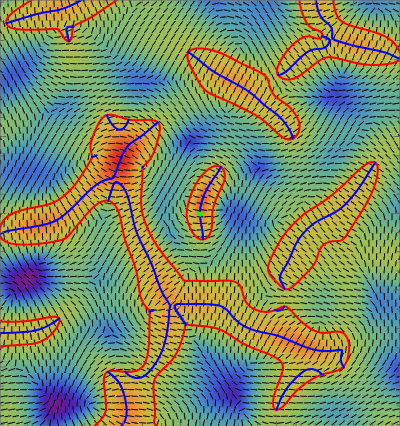
\includegraphics[width=\textwidth]{Cusp_L}
\end{subfigure}~
\begin{subfigure}[b]{0.3\textwidth}
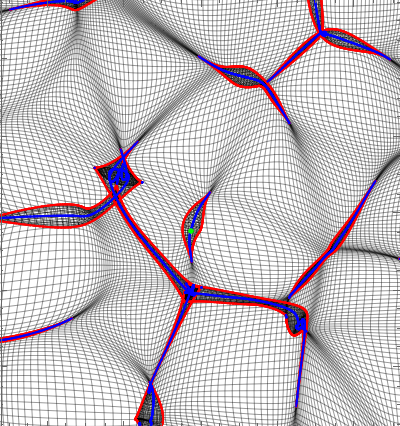
\includegraphics[width=\textwidth]{Cusp_Z}
\end{subfigure}~
\begin{subfigure}[b]{0.3\textwidth}
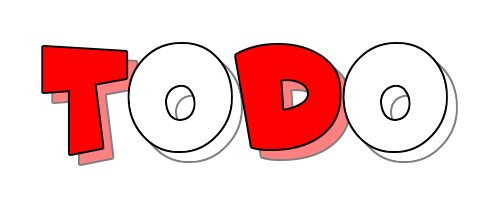
\includegraphics[width=\textwidth]{Todo}
\end{subfigure}\\
%%%%%%%%%%
%%%%%%%%%%
\begin{subfigure}[b]{0.3\textwidth}
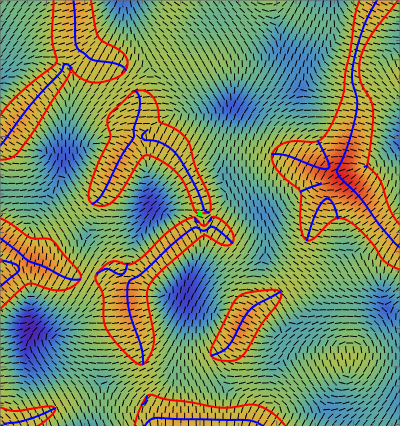
\includegraphics[width=\textwidth]{Swallowtail_L}
\end{subfigure}~
\begin{subfigure}[b]{0.3\textwidth}
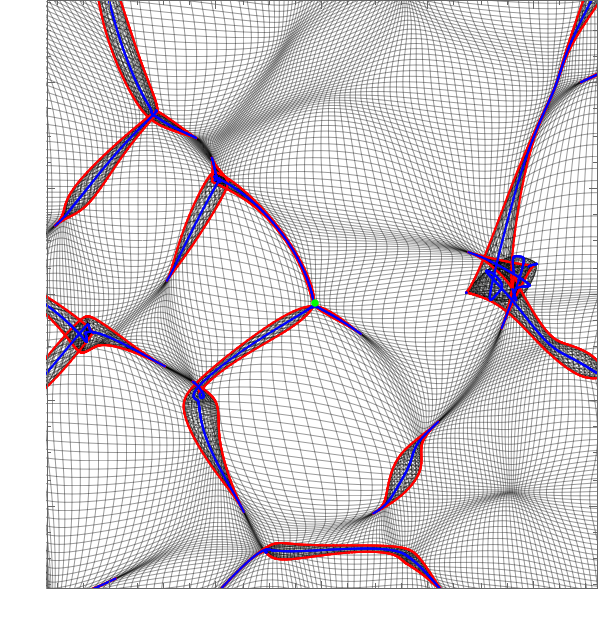
\includegraphics[width=\textwidth]{Swallowtail_Z}
\end{subfigure}~
\begin{subfigure}[b]{0.3\textwidth}
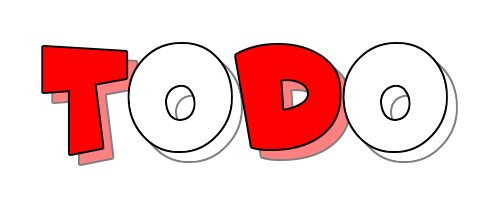
\includegraphics[width=\textwidth]{Todo}
\end{subfigure}\\
%%%%%%%%%%
%%%%%%%%%%
\begin{subfigure}[b]{0.3\textwidth}
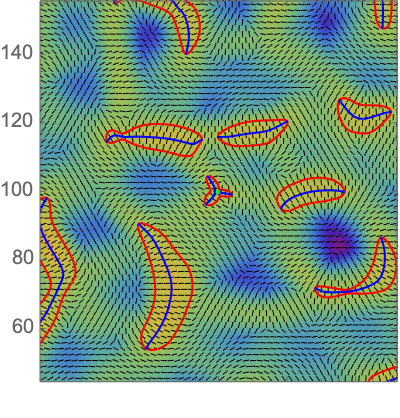
\includegraphics[width=\textwidth]{Elliptic_L}
\end{subfigure}~
\begin{subfigure}[b]{0.3\textwidth}
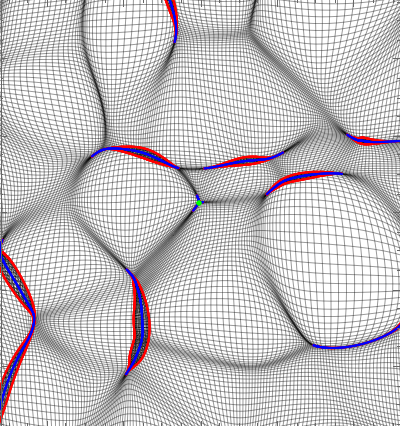
\includegraphics[width=\textwidth]{Elliptic_Z}
\end{subfigure}~
\begin{subfigure}[b]{0.3\textwidth}
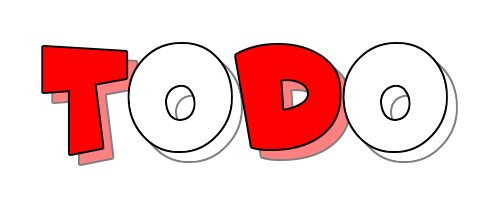
\includegraphics[width=\textwidth]{Todo}
\end{subfigure}\\
%%%%%%%%%%
%%%%%%%%%%
\begin{subfigure}[b]{0.3\textwidth}
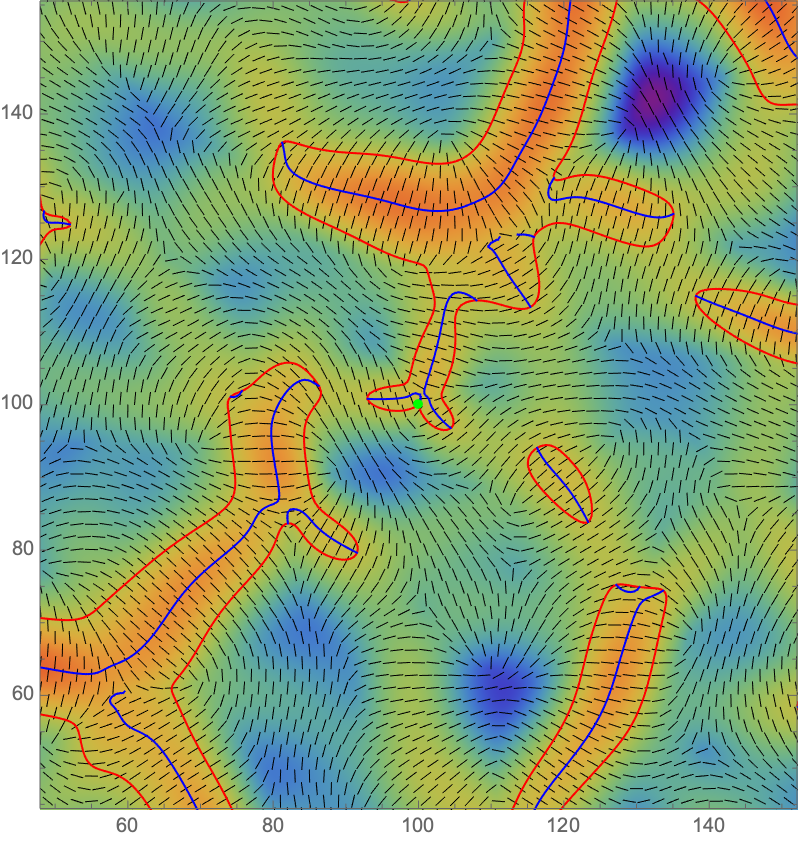
\includegraphics[width=\textwidth]{Hyperbollic_L}
\end{subfigure}~
\begin{subfigure}[b]{0.3\textwidth}
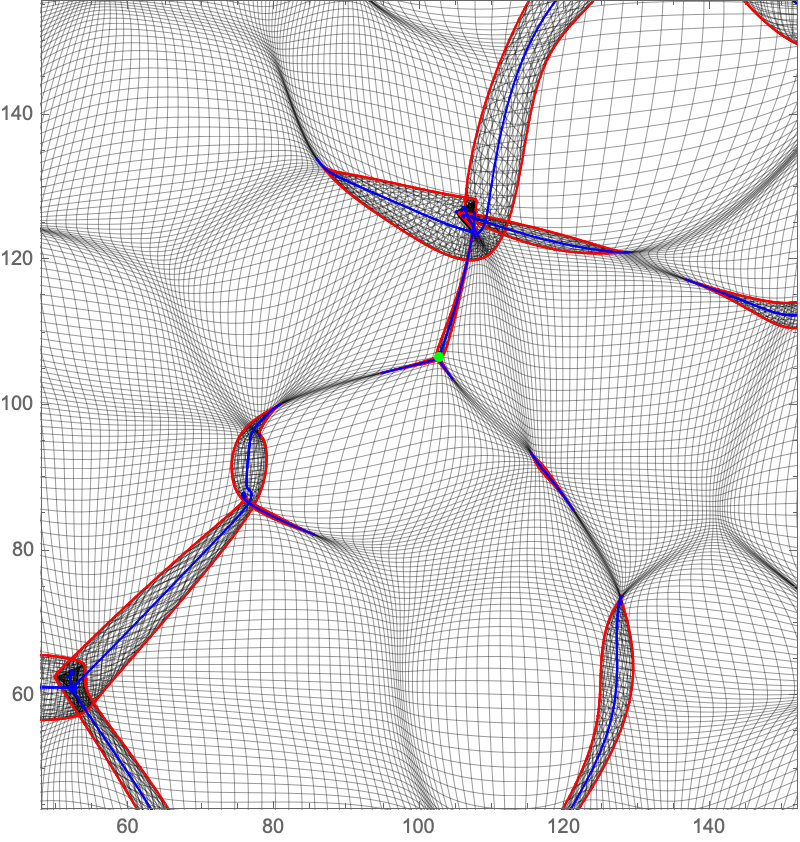
\includegraphics[width=\textwidth]{Hyperbollic_Z}
\end{subfigure}~
\begin{subfigure}[b]{0.3\textwidth}
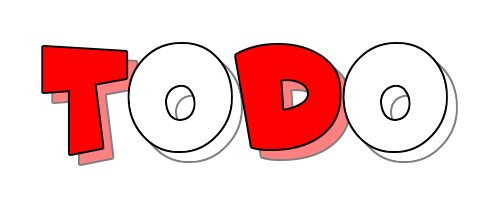
\includegraphics[width=\textwidth]{Todo}
\end{subfigure}
\caption{Elements of the caustic skeleton. \textit{From top to bottom:} the cusp, the swallowtail, the elliptic and the hyperbolic caustic. \textit{Left:} the caustic skeleton in Lagrangian space. \textit{Centre:} the Zel'dovich approximation. \textit{Right:} the $N$-body simulation {\color{red}(To Do)}.}\label{fig:caustics_Examples_Big}
\end{figure}

%%%%%%%%%%%%%%%%%%%%%%%%%%%%%%%%%%%%%%%%%%%%%%%%%%%%%%%%%%%%%%%%
\subsection{The Zel'dovich approximation}\label{sec:Zeldovich}
In this paper we define the caustic skeleton using the Zel'dovich approximation and study the resulting structures using a dark matter $N$-body simulation. The Zel'dovich approximation is the first order approximation in Lagrangian fluid dynamics, for which the displacement field factorizes into a spatial and a temporal part
\begin{align}
\bm{s}_t(\bm{q}) = - b_+(t) \nabla_{\bm{q}} \Psi(\bm{q})\,.
\end{align}
The growing mode $b_+(t)$ is a natural time parameter satisfying the differential equation
\begin{align}
\frac{\mathrm{d}^2 b_+(t)}{\mathrm{d}t^2} + 2 \frac{\dot{a}(t)}{a(t)} \frac{\mathrm{d} b_+(t)}{\mathrm{d}t} = 4 \pi G \rho_u(t) b_+(t)\,.
\end{align}
The displacement potential $\Psi$ captures the geometry of the cosmic web, and is proportional to the primordial gravitational potential
\begin{align}
\Psi(\bm{q}) &=\frac{1}{4 \pi G a^2 \rho_0}\phi_0(\bm{q})%\\
%&= \frac{2}{3\Omega_0 H_0^2}\phi_0(\bm{q})
\,,
\end{align}
expressed in terms of the current total energy density %$\Omega_0$ and
$\rho_0$,
%the current Hubble parameter $H_0$,
and the linearly extrapolated gravitational potential $\phi_0$. Note that the Poisson equation relates the primordial gravitational potential to the primordial density perturbation
\begin{align}
\nabla ^2 \phi_0 &= 4 \pi G a^2 \rho_u \delta_0\,.%\\
%&= \frac{3}{2} \Omega H^2 a^2 \delta\,,
\end{align}
In the Zel'dovich approximation, the mass elements follow linear trajectories that are completely determined by the primordial gravitational potential. The approximation accurately describes single-stream regions but fails when mass streams overlap and gravitational interactions between mass elements become important. When working with the Zel'dovich approximation, it is convenient to work in terms of the Hessian of the displacement potential,
\begin{align}
\bm{\psi}=\mathcal{H}\Psi\,,
\end{align}
and the corresponding eigenvalue $\lambda_i$ and $\bm{v}_i$
\begin{align}
\bm{\psi}\bm{v}_i = \lambda_i \bm{v}_i
\end{align}
with the relation $\lambda_1 =-\mu_2/b_+,\lambda_2 =-\mu_1/b_+$, assuming the ordering $\lambda_1(\bm{q}) \geq \lambda_2(\bm{q})$. In terms of the eigenvalue fields $\lambda_i$, the density takes the form 
\begin{align}
\rho_t(\bm{x})
&= \sum_{\bm{q} \in A_t(\bm{x})} \frac{\bar{\rho}}{|1-b_+(t) \lambda_1(\bm{q})||1-b_+(t) \lambda_2(\bm{q})|}\,.
\end{align}
Initially, the growing mode $b_+$ vanishes and the universe consists of a single-stream region. As the fluid collapses under self gravity, the growing mode $b_+$ increases. The fold caustics form at the level sets of the eigenvalue field $\{\bm{q}|\lambda_i(\bm{q})=1/b_+(t)\}$. From this picture we observe the direct connection between the critical points of the eigenvalue fields and the connectivity of the cosmic web.


%%%%%%%%%%%%%%%%%%%%%%%%%%%%%%%%%%%%%%%%%%%%%%%%%%%%%%%%%%%%%%%%
\subsection{Caustics in the cosmic web}

\begin{figure}
\centering
\begin{subfigure}[b]{0.24\textwidth}
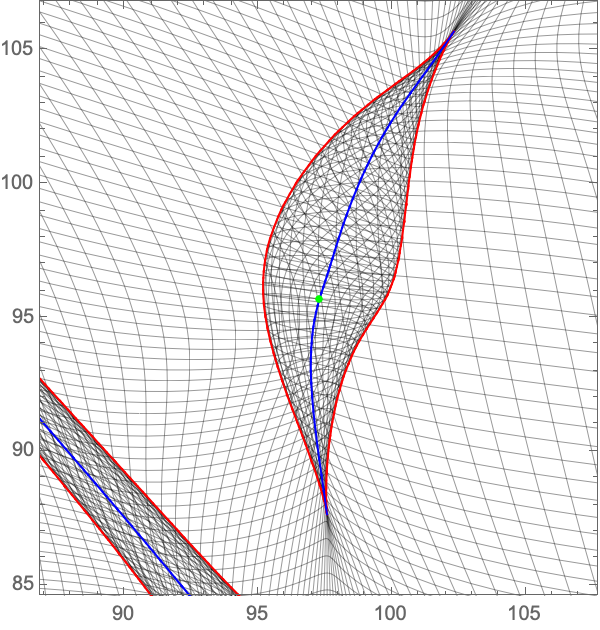
\includegraphics[width=\textwidth]{Cusp_Z_Zoom}
\end{subfigure}~
\begin{subfigure}[b]{0.24\textwidth}
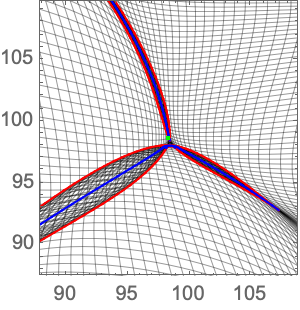
\includegraphics[width=\textwidth]{Swallowtail_Z_Zoom}
\end{subfigure}~
\begin{subfigure}[b]{0.24\textwidth}
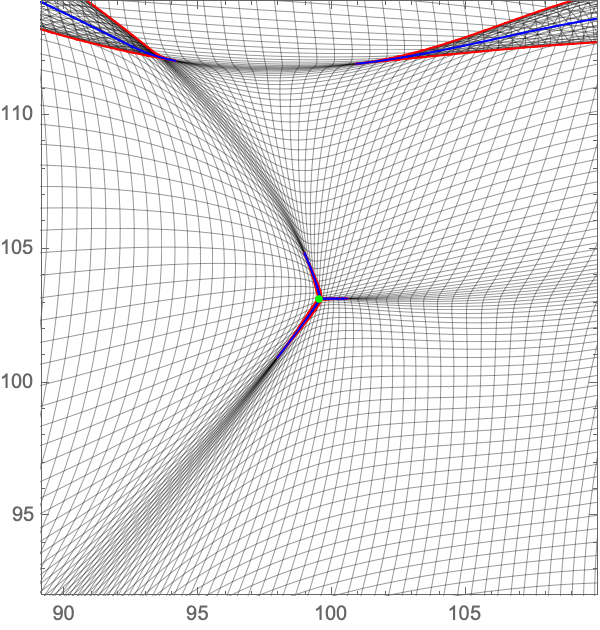
\includegraphics[width=\textwidth]{Elliptic_Z_Zoom}
\end{subfigure}~
\begin{subfigure}[b]{0.24\textwidth}
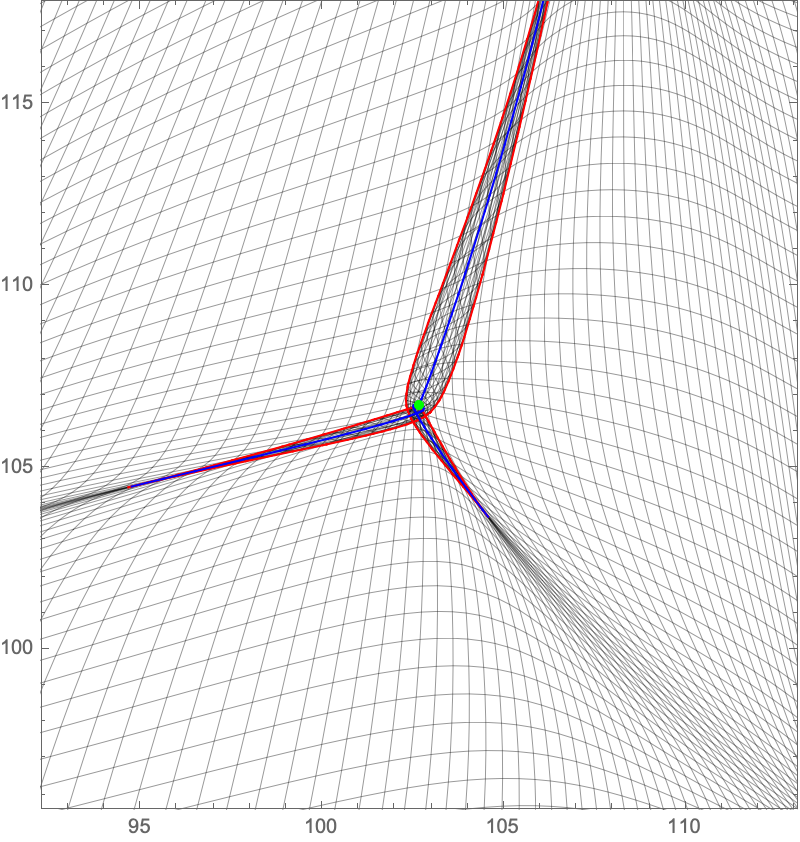
\includegraphics[width=\textwidth]{Hyperbollic_Z_Zoom}
\end{subfigure}\\
\begin{subfigure}[b]{0.24\textwidth}
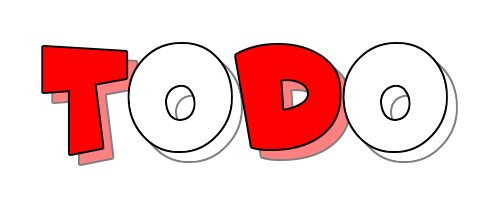
\includegraphics[width=\textwidth]{Todo}
\end{subfigure}~
\begin{subfigure}[b]{0.24\textwidth}
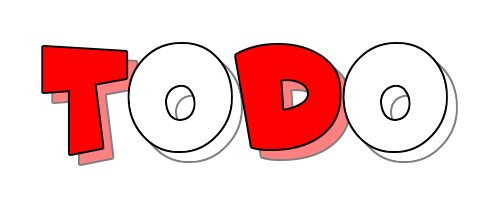
\includegraphics[width=\textwidth]{Todo}
\end{subfigure}~
\begin{subfigure}[b]{0.24\textwidth}
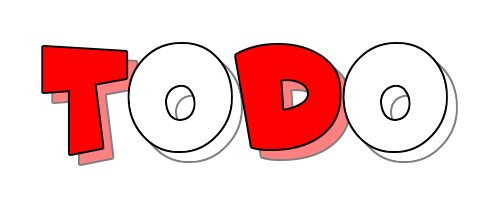
\includegraphics[width=\textwidth]{Todo}
\end{subfigure}~
\begin{subfigure}[b]{0.24\textwidth}
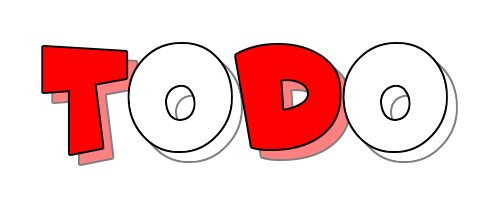
\includegraphics[width=\textwidth]{Todo}
\end{subfigure}
\caption{Zoom in with a $(20 \text{ Mpc})^2$ box centred around the caustic. From left to right, we see the cusp, the swallowtail, the elliptic umbilic, and the hyperbollic umbilic caustics. The upper and lower panels display the Zel'dovich approximation and the $N$-body simulation.}\label{fig:caustics_Examples_Small}
\end{figure}

The role of the different elements of the caustic skeleton can be clearly observed from the zoom of figure \ref{fig:caustics_Examples_Big} centered on the caustic in Lagrangian space (see figure \ref{fig:caustics_Examples_Small}). Observe that the cusp curve bisects the multi-stream region, marking the location where the mass elements turn around to form a line-like structure. The swallowtail, elliptic and hyperbolic caustics form where different cusp curves meet up to form a knot. The swallowtail caustic marks the place where the cusp curve corresponding to a single eigenvalue field becomes non-differentiable. The elliptic and hyperbolic caustics mark the location where the multi-stream regions of different eigenvalue fields merge. Since the formation history of these different point caustics differs, it is natural to expect the properties of the different clusters to vary in nature. Note that the cluster caustics are rarely isolated. They will generally cluster and form an intricate multi-stream structure. This way, a cluster can connect more than three filaments.

\begin{framed}
{\color{red} I will expand this section a bit once we have the N-body simulation.}
\end{framed}





%%%%%%%%%%%%%%%%%%%%%%%%%%%%%%%%%%%%%%%%%%%%%%%%%%%%%%%%%%%%%%%%
\section{Constrained random field theory}\label{sec:GRF}
One of the most startling realizations in modern cosmology is that the intricate cosmic web, observed in several cosmological redshift surveys, originated from extremely simple initial conditions. At the moment of recombination, when the baryons and electrons form neutral elements and decouple from the photons, the energy density in our universe $\rho(\bm{q})$, was extremely homogeneous. These fluctuations -- commonly expressed in terms of the perturbations
\begin{align}
\delta(\bm{q}) = \frac{\rho(\bm{q})}{\bar{\rho}} -1\,,
\end{align}
with the mean density $\bar{\rho} = \langle \rho \rangle$ -- left an imprint as temperature fluctuations in the Cosmic Microwave Background field (CMB) which, over the last decades, have been measured with increasing accuracy. After recombination, the pressure dropped and these small density fluctuations started to collapse under the force of gravity. This led to the rich geometric patterns in the cosmic web and virialized objects we observe today. The statistical properties of these initial perturbations $\delta$, is very close to Gaussian. We here define Gaussian random fields and discuss the implementation of both linear and non-linear constraints.

\begin{framed}
The mathematics of Gaussian random fields is surprisingly close to Euclidean path integrals in statistical field theory. We believe that it will prove useful to apply well-established concepts from statistical field theory to the exploration of the fundaments of the cosmic web.
\end{framed}

%%%%%%%%%%%%%%%%%%%%%%%%%%%%%%%%%%%%%%%%%%%%%%%%%%%%%%%%%%%%%%%%
\subsection{Gaussian random fields}
A two-dimensional Gaussian random field $f:\mathbb{R}^2\to \mathbb{R}$ is a continuous generalization of a multi-dimensional normal distribution, defined by the probability density
\begin{align}
p(\delta) = \mathcal{N} e^{- S[f]}\,, \label{eq:functional_Distribution}
\end{align}
with the normalization constant $\mathcal{N}$ and the `action' (in analogy with the Euclidean path integral)
\begin{align}
S[f]\equiv \frac{1}{2} \iint (f(\bm{q}_1) - \bar{f}(\bm{q}_1)) K(\bm{q}_1,\bm{q}_2) (f(\bm{q}_2) -\bar{f}(\bm{q}_2))\mathrm{d}\bm{q}_1 \mathrm{d}\bm{q}_2,\label{eq:action}
\end{align}
defined in terms of the mean field $\bar{f}(\bm{q})$ and the kernel $K(\bm{q}_1,\bm{q}_2)$. The probability that the random field $f$ is included in a set of functions $\mathcal{S}$ is defined by the path integral
\begin{align}
P[f \in \mathcal{S}] = \mathcal{N} \int \bm{1}_\mathcal{S}(f) e^{-S[f]}\,\mathcal{D}f\,,
\end{align}
with $\bm{1}_\mathcal{S}$ the identity function\footnote{Defined by $\bm{1}_\mathcal{S}(x)=1$ when $x \in \mathcal{S}$ and $\bm{1}_\mathcal{S}(x)=0$ when $x \notin \mathcal{S}$.} and $\mathcal{D}f$ the path integral measure. The expectation value of a functional $Q[f]$ is given by
\begin{align}
\left\langle Q[f] \right\rangle = \mathcal{N}\int Q[f]\, e^{-S[f]}\,\mathcal{D}f\,,
\end{align}
analogous to Euclidean path integrals in statistical field theory. It can be shown that the expectation value of the random field is given by the mean field
\begin{align}
\langle f(\bm{q})\rangle &= \bar{f}(\bm{q})\,.
\end{align}
Two-point correlation function
\begin{align}
\xi(\bm{q}_1, \bm{q}_2) &= \langle (f(\bm{q}_1) - \bar{f}(\bm{q}_1)) (f(\bm{q}_2) - \bar{f}(\bm{q}_2))\rangle\\
&= \int (f(\bm{q}_1) - \bar{f}(\bm{q}_1)) (f(\bm{q}_2) - \bar{f}(\bm{q}_2)) e^{-S[f]}\mathcal{D}f
\end{align}
is the inverse of the two-point correlation function,
\begin{align}
\int K(\bm{q}_1,\bm{q}) \xi(\bm{q},\bm{q}_2) \mathrm{d}\bm{q}= \delta_D^{(2)}(\bm{q}_1-\bm{q}_2)\,,\label{eq:defK}
\end{align}
with the two-dimensional Dirac delta function $\delta_D^{(2)}$. The Gaussian random field is thus fully determined by the mean field $\bar{f}$ and the two-point correlation function $\xi$. 

In cosmology, the cosmological principle often leads to the study of statistically homogeneous and isotropic random fields for which the mean field is constant $\bar{f}(\bm{q})=\bar{f}$ and the two point correlation function only depends on the magnitude of the difference of the inserted points, \textit{i.e.}, $\xi(\bm{q}_1,\bm{q}_2)=\xi(\|\bm{q}_1-\bm{q}_2\|)$, and consequently $K(\bm{q}_1,\bm{q}_2)=K(\|\bm{q}_1-\bm{q}_2\|)$. We will in particular consider random fields with vanishing means $\bar{f}=0$. 

The statistical properties of homogeneous and isotropic random fields are most transparently expressed in terms of the Fourier transformation of the random field
\begin{align}
\hat{f}(\bm{k}) = \int f(\bm{x})e^{i\bm{k}\cdot \bm{x}}\mathrm{d}\bm{x}\,.
\end{align}
Note that the Fourier modes of real-valued Gaussian random fields satisfy the reality condition $\hat{f}(\bm{k}) = \hat{f}^*(-\bm{k})$. Using the double convolution theorem, we express the action \eqref{eq:action} as
\begin{align}
S[f] = \frac{1}{2} \int |\hat{f}(\bm{k})|^2 \hat{K}(\bm{k}) \frac{\mathrm{d}\bm{k}}{(2\pi)^2}\,.
\end{align}
In Fourier space, equation \eqref{eq:defK} takes the form
\begin{align}
\int \hat{K}(\bm{k}) P(\bm{k}) e^{i\bm{k}(\bm{x}_1-\bm{x}_2)} \frac{\mathrm{d}\bm{k}}{(2\pi)^2} = \delta_D^{(2)}(\bm{x}_1 - \bm{x}_2)\,,
\end{align}
with the power spectrum defined as the Fourier transform of the two-point correclation function,
\begin{align}
P(\bm{k}) = \int \xi(\bm{x}) e^{i\bm{k}\bm{x}}\mathrm{d}\bm{x}\,,
\end{align}
implying the relation $\hat{K}(\bm{k}) = 1/P(\|\bm{k}\|)$. The resulting probability density of the Fourier modes is diagonal
\begin{align}
p(\hat{f}) \propto \exp\left[ -\frac{1}{2} \int \frac{|\hat{f}(\bm{k})|^2}{P(\|\bm{k}\|)} \frac{\mathrm{d}\bm{k}}{(2\pi)^2}\right]\,,
\end{align}
implying the covariance
\begin{align}
\langle \hat{f}(\bm{k}_1)\hat{f}(\bm{k}_2) \rangle = (2\pi)^2 \delta_D^{(2)}(\bm{k}_1-\bm{k}_2) P(\|\bm{k}_1\|)\,.
\end{align}

In practice, we often we often consider realizations of Gaussian random fields on a lattice, or more generally a finite set of linear statistics $\bm{Y}=(Y_1,Y_2,\dots,Y_M)$. In this setting, the functional distribution \eqref{eq:functional_Distribution} reduces to the multi-dimensional Gaussian distribution,
\begin{align}
p(\bm{Y}) = \frac{\exp\left[-\frac{1}{2} \sum_{i,j}^n \Delta \bm{Y}^T M^{-1} \Delta \bm{Y}\right]}{[(2\pi)^n \det M]^{1/2}}\,,
\end{align}
with the deviation from the mean $\Delta \bm{Y} = \bm{Y} - \langle \bm{Y}\rangle$ and the covariance matrix
\begin{align}
M = \text{cov}(\bm{Y},\bm{Y}) = \langle \Delta \bm{Y}^T \Delta \bm{Y}\rangle\,.
\end{align}


%%%%%%%%%%%%%%%%%%%%%%%%%%%%%%%%%%%%%%%%%%%%%%%%%%%%%%%%%%%%%%%%
\subsubsection{Generating realizations}

The distribution of the discrete Fourier modes $\bm{Y}(\hat{f}(\bm{k}_1),\hat{f}(\bm{k}_1),\dots)$ takes the form 
\begin{align}
p(\hat{f}(\bm{k}_1), \hat{f}(\bm{k}_2), \dots) = \prod_{i} \frac{1}{\sqrt{2\pi P(\| \bm{k}_i\|)}} e^{-\frac{|\hat{f}(\bm{k}_i)|^2}{2P(\|\bm{k}_i\|)}},
\end{align}
yielding an efficient method to generate realizations. Firstly, generate Gaussian white noise on a lattice with zero mean and unit standard deviation. Secondly, Fourier transform the lattice with a FFT routine and multiply the resulting field with the square root of the power spectrum $\sqrt{P(\bm{k})}$. Finally, perform a inverse Fourier transform to obtain a realization of the random field.


\begin{framed}
{\color{red} I am not yet sure where to place this section. }\\

The statistical properties of these random fields are often conveniently expressed in terms of the moments
\begin{align}
\sigma_i^2 &= \frac{1}{(2\pi)^2} \int \|\bm{k}\|^{2i}P(\|\bm{k}\|)\mathrm{d}\bm{k}\nonumber\\
&= \frac{1}{2\pi} \int_0^\infty k^{2i+1}P(k)\mathrm{d}k\,,
\end{align}
with the magnitude $k = \|\bm{k}\|$.
\end{framed}

%%%%%%%%%%%%%%%%%%%%%%%%%%%%%%%%%%%%%%%%%%%%%%%%%%%%%%%%%%%%%%%%
\subsection{Linear constraints: Gaussian fields}
In this paper, we study how the different geometric features of the cosmic web emerge from different initial conditions. To systematically study these initial conditions we use constrained Gaussian random field theory. In this section, we develop the theory of linear constraints following the analysis of [van de Weygaert and Bertschinger 1996]. In the next section, we generalize this discussion to a large class of non-linear constraints. We restrict both discussions to statistically homogeneous and isotropic fields with vanishing mean.

For a random field $f$, consider a set of linear constraints
\begin{align}
\Gamma =\{ C_i[f;\bm{q}_i] = c_i,\,\ i=1,\dots,M \}\,,
\end{align}
with the linear functional $C_i[f;\bm{q}]$ assuming the value $c_i$ in $\bm{q}_i$. A linear functional can take the form of the function value at a point
\begin{align}
C[f;\bm{q}'] &= f(\bm{q}')\,,
\end{align}
its derivative at a point
\begin{align}
C[f;\bm{q}'] &= \frac{\partial}{\partial q_i}f(\bm{q}')\,,
\end{align}
or more generally a convolution
\begin{align}
C[f;\bm{q}'] &= \int g(\bm{q}' - \bm{q})f(\bm{q})\mathrm{d}\bm{q}\,,
\end{align}
with the convolution kernel $g$. 

The constraint random field follows the distribution
\begin{align}
p(f|\Gamma) = \frac{p(f,\Gamma)}{p(\Gamma)}\,,
\end{align}
where the constraints follow the Gaussian marginal distribution
\begin{align}
p(\Gamma) = \frac{\exp\left[-\frac{1}{2} \Delta\bm{C}^T Q^{-1} \Delta\bm{C} \right]}{[(2\pi)^M \det Q]^{1/2}}\,,
\end{align}
with the vector $\bm{C}=(C_1[f;\bm{q}_1], \dots, C_M[f;\bm{q}_M])$ and the covariance matrix $Q = \text{cov}(\bm{C}, \bm{C})$. The constraint distribution can written in terms of the Gaussian probability density
\begin{align}
p(f|\Gamma) \propto  e^{-\frac{1}{2} \left[\iint f(\bm{q}_1) K(\|\bm{q}_1 - \bm{q}_2\|) f(\bm{q}_2)\mathrm{d}\bm{q}_1 \mathrm{d}\bm{q}_2 -\Delta \bm{C}^TQ^{-1}\Delta \bm{C}\right]},\label{eq:constraint1}
\end{align}
in the space of functions satisfying the constraints $\Gamma$.

In appendix \ref{ap:constraintDensity}, we derive the mean field
\begin{align}
\langle f(\bm{q})|\Gamma\rangle = \sum_{i,j=1}^M\xi_i (\bm{q})\xi_{ij}^{-1}c_j\,,
\end{align}
and the covariance
\begin{align}
\text{cov}(f(\bm{q}_1),f(\bm{q}_2)|\Gamma)  = \xi(\bm{q}_1,\bm{q}_2) - \sum_{i,j=1}^M\xi_i(\bm{q}_1)\xi_{ij}^{-1}\xi_j(\bm{q}_2)\,,
\end{align}
with the covariance of the random field and the constraints $\xi_{i}(\bm{q}) = \text{cov}( f(\bm{q}), C_i)$ and the constraints $\xi_{ij} = \text{cov}( C_i ,C_j)$. Note that the covariance is independent of the values $\bm{c}$ the constraints $\bm{C}$ assume. This is a special property of Gaussian distributions. Consequently, the probability density takes the form
\begin{align}
p(f|\Gamma) \propto  e^{-\frac{1}{2} \iint \delta{f}(\bm{q}_1) \tilde{K}(\bm{q}_1,\bm{q}_2) \delta f(\bm{q}_2)\mathrm{d}\bm{q}_1 \mathrm{d}\bm{q}_2 }\,,\label{eq:constraint2}
\end{align}
with the residue $\delta f = f-\langle f(\bm{q})|\Gamma\rangle$ and the constrained kernel $\tilde{K}$ defined as the inverse of the constrained two-point correlation function, \textit{i.e.},
\begin{align}
\int \tilde{K}(\bm{q}_1,\bm{q}) \left[\xi(\bm{q},\bm{q}_2) - \sum_{i,j=1}^M\xi_i(\bm{q})\xi_{ij}^{-1}\xi_j(\bm{q}_2)\right]\mathrm{d}\bm{q}= \delta_D^{(2)}(\bm{q}_1-\bm{q}_2)\,.
\end{align}
Note that earlier papers [REFS] worked in the space of functions satisfying the constraints $\Gamma$, neglecting the correction $\sum_{i,j=1}^M\xi_i(\bm{q})\xi_{ij}^{-1}\xi_j(\bm{q}_2)$, and using the original kernel $K$ for the residue. In this study, we prefer to work in space of unrestricted functions, as the correction makes the inhomogeneity and anisotropy of the residue manifest. These properties are most clearly observed in the variance of the residue,
\begin{align}
\langle \delta f(\bm{q})^2|\Gamma \rangle = \sigma_0^2- \sum_{i,j=1}^M\xi_i(\bm{q})\xi_{ij}^{-1}\xi_j(\bm{q})\,,
\end{align}
which vanishes on the constraints. Away from the constraints, the variance of the residue approaches the variance of the unconstrained  field $\text{var}(f)=\sigma_0^2$.

To judge the relevance of a particular set of constraints, it is useful to evaluate the $\chi^2$ of the set of values $c_i$,
\begin{align}
\chi^2 = \sum_{i,j=1}^M c_i\, \xi_{ij}^{-1}c_j.
\end{align}
The probability that this constraint yields a $\chi^2$ higher than the this number is given by $\Gamma_Q(M/2, \chi^2/2)$ with the incomoplete gamma function $\Gamma_Q$.

%%%%%%%%%%%%%%%%%%%%%%%%%%%%%%%%%%%%%%%%%%%%%%%%%%%%%%%%%%%%%%%%
\subsubsection{Generating realizations}
The Hoffman-Ribak method cleverly uses the property that the statistics of the residue $\delta f$ are independent of $c_i$, to generate realizations of the constraint Gaussian random field. Firstly, generate a realization $g$ of the unconstraint Gaussian random field with the required power spectrum. Secondly, evaluate the constraints for this realization $C_i[g;\bm{q}'_i]=d_i$ and the corresponding mean field $\bar{g}$. The statistical properties of the residue with respect to this mean field $\delta g = g-\bar{g}$ are independent of the value the constraints assume and thus identical to the properties of the residue $\delta f$. We can thus identify the residue of the field $g$ with the residue of the constrained field $f$. By adding the residue of the unconstraint field to the mean field with the required constraints, we obtain the realization of the constrained Gaussian random field.



%%%%%%%%%%%%%%%%%%%%%%%%%%%%%%%%%%%%%%%%%%%%%%%%%%%%%%%%%%%%%%%%
\subsection{Non-linear constraints: formalism}
For the systematic investigation of the caustic skeleton, we extend constraint Gaussian random field theory to include non-linear constraints. More specifically, we extend the theory of linear constraints to the large class of non-linear constraints expressed in terms of a finite number of linear statistics.

Consider the set of linear functionals $C_i[f,\bm{q}_i]$ with $i=1,\dots,M$ and the space of values $\bm{c}=(c_1,\dots,c_M)$ the linear functionals can assume $\mathbb{R}^M$. On this space, we define a set of functions $\mathcal{C}_i:\mathbb{R}^M \to \mathbb{R}$ with $i=1,\dots,N$ and $N\leq M$, and the non-linear constraint $\Gamma = \{\mathcal{C}_i(\bm{C}) = 0\}_{i=1}^N$. We can visualize this geometrically by considering the $(M-N)$-dimensional constraint manifold $\mathcal{M}_\mathcal{C}$ in the space of the $M$ linear constraints
\begin{align}
\mathcal{M}_{\mathcal{C}} = 
\{\bm{c}\, |\, \mathcal{C}_i(\bm{c}) = 0 \text{ for all } i=1,\dots,N\}.
\end{align}
See figure \ref{fig:constraintManifold} for a sketch of this constraint manifold. On this manifold $\mathcal{M}_\mathcal{C}$, the constraint probability density is proportional to the original Gaussian distribution
\begin{framed}
\begin{align}
p(\bm{c}\,|\,\bm{c}\in \mathcal{M}_{\mathcal{C}})  = \frac{p(\bm{c})}{\int_{\mathcal{M}_\mathcal{C}} p(\bm{c})\, \mathrm{d}\bm{c}}\,.
\end{align}
\end{framed}
Note that the curvature of $\mathcal{M}_\mathcal{C}$ generally makes the induced density $p(\bm{c}\,|\,\bm{c}\in \mathcal{M}_{\mathcal{C}})$ non-Gaussian. We extend constraint Gaussian random field theory to include non-linear constraints by studying the finite dimensional probability density $p(\bm{c}\,|\,\bm{c}\in \mathcal{M}_{\mathcal{C}})$.



\begin{figure}
\centering
\begin{subfigure}[b]{0.49\textwidth}
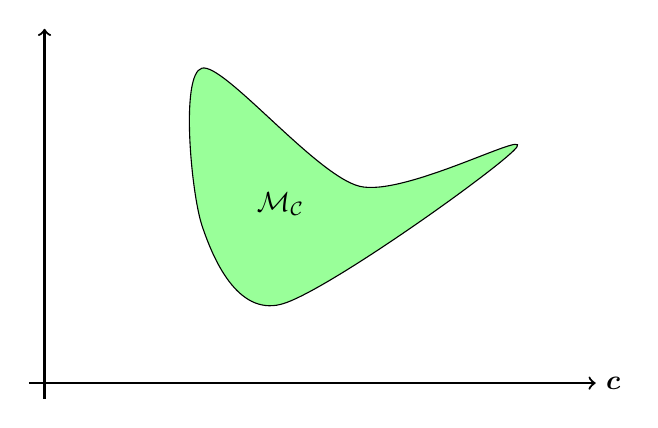
\begin{tikzpicture}
%\draw[draw=black] (0,0) rectangle ++(7,5);
\draw[->, thick] (-0.2,0)--(7,0) node[right]{$\bm{c}$};
\draw[->, thick] (0,-0.2)--(0,4.5);
%\draw [fill=blue!80] plot [mark=none, smooth cycle] coordinates {(2,2) (3,1) (6,3) (4,2.5) (2,4)};
\draw [fill=green!40] plot [mark=none, smooth cycle] coordinates {(2,2) (3,1) (6,3) (4,2.5) (2,4)};
%\draw [fill=lime!70] plot [mark=none, smooth cycle] coordinates {(2,2) (3,1) (6,3) (4,2.5) (2,4)};
\node[above] at (3,2) {$\mathcal{M}_\mathcal{C}$};
\end{tikzpicture}
\end{subfigure}
\caption{The constraint manifold $\mathcal{M}_\mathcal{C}$ in the space of linear constraint values.}\label{fig:constraintManifold}
\end{figure}


\begin{itemize}
\item
The problem of generating realizations of the more general constraints fields is reduced to sampling realizations of the distribution $p(\bm{c}|\bm{c}\in \mathcal{M}_\mathcal{C})$, using the Hoffman-Ribak method.

\item
The mean field of takes the surprisingly simple form 
\begin{framed}
\begin{align}
\bar{f}_{\mathcal{C}}(\bm{q}) =\bar{f}_{\bar{\bm{c}}}(\bm{q})\,
\end{align}
\end{framed}
with the mean constraint
\begin{align}
\bar{\bm{c}} &\equiv \langle \bm{c} \,|\, \Gamma\rangle = \int_{\bm{c} \in \mathcal{M}_{\mathcal{C}}}  \bm{c}\, p(\bm{c}\,|\,\bm{c}\in \mathcal{M}_{\mathcal{C}}) \mathrm{d}\bm{c}\,,
\end{align}
from the realization that 
\begin{align}
\bar{f}_{\mathcal{C}}(\bm{q}) 
&=\left\langle f(\bm{q})|\Gamma\right \rangle \nonumber\\
&= \int_{\bm{c} \in \mathcal{M}_{\mathcal{C}}} \bar{f}_{\bm{c}}(\bm{q})\, p(\bm{c}|\bm{c}\in \mathcal{M}_{\mathcal{C}}) \mathrm{d}\bm{c}\nonumber\\
&= \sum_{i,j=1}^n\xi_i(\bm{q}) \xi_{ij}^{-1}\int_{\bm{c} \in \mathcal{M}_{\mathcal{C}}}  c_i\, p(\bm{c}|\bm{c}\in \mathcal{M}_{\mathcal{C}}) \mathrm{d}\bm{c}\nonumber\\
&= \sum_{i,j=1}^n \xi_i(\bm{q}) \xi_{ij}^{-1} \bar{c}_i\nonumber\\
&= \bar{f}_{\bar{\bm{c}}}(\bm{q})\,.
\end{align}

\item
The variance of the corresponding residue, $\delta f = f - \bar{f}_{\mathcal{C}}$, coincides with the variance of residue of the corresponding constraint problem with linear constraints
\begin{framed}
\begin{align}
\left \langle \delta f (\bm{q})^2\,|\,\Gamma\right\rangle =
\sigma_0^2 - \sum_{i,j=1}^M\xi_i(\bm{q}) \xi_{ij}^{-1} \xi_j(\bm{q}) + \sum_{i,j,k,l=1}^M \xi_{i}(\bm{q})\xi_{ij}^{-1}\xi_{k}(\bm{q})\xi_{kl}^{-1}\text{cov}(c_j, c_l|\bm{c}\in\mathcal{M}_\mathcal{C})
\,,
\end{align}
\end{framed}
where $\text{cov}(c_j, c_l|\bm{c}\in\mathcal{M}_\mathcal{C})$ captures the geometry of the constraint manifold $\mathcal{M}_\mathcal{C}$, following directly from
\begin{align}
\left \langle \delta f (\bm{q})^2\,|\,\Gamma\right\rangle 
&= \int_{\mathcal{M}_\mathcal{C}} \langle (f(\bm{q})-\bar{f}_{\bar{\bm{c}}}(\bm{q}))^2|C_i[f,\bm{q}_i]=c_i\rangle p(\bm{c}|\bm{c}\in\mathcal{M}_{\mathcal{C}})\mathrm{d}\bm{c}\\
&= \int_{\mathcal{M}_\mathcal{C}} \langle f^2(\bm{q})|C_i[f,\bm{q}_i]=c_i\rangle p(\bm{c}|\bm{c}\in\mathcal{M}_{\mathcal{C}})\mathrm{d}\bm{c} - \bar{f}_{\bar{\bm{c}}}^2(\bm{q})\\
&= \int_{\mathcal{M}_\mathcal{C}} \langle (f(\bm{q})-\bar{f}_{\bm{c}}(\bm{q}))^2|C_i[f,\bm{q}_i]=c_i\rangle p(\bm{c}|\bm{c}\in\mathcal{M}_{\mathcal{C}})\mathrm{d}\bm{c} \\
&\ \ +\int_{\mathcal{M}_\mathcal{C}} (\bar{f}_{\bm{c}}(\bm{q})- \bar{f}_{\bar{\bm{c}}}^2(\bm{q}))^2p(\bm{c}|\bm{c}\in\mathcal{M}_{\mathcal{C}})\mathrm{d}\bm{c} \\
&=  \sigma_0^2 - \sum_{i,j=1}^M\xi_i(\bm{q}) \xi_{ij}^{-1} \xi_j(\bm{q}) + \sum_{i,j,k,l=1}^M \xi_{i}(\bm{q})\xi_{ij}^{-1}\xi_{k}(\bm{q})\xi_{kl}^{-1}\text{cov}(c_j, c_l|\bm{c}\in\mathcal{M}_\mathcal{C})\,.
\end{align}
Note that the variance of the residue with respect to the non-linear constraint is no longer independent of the values the constraint assumes. When $\mathcal{M}_\mathcal{C}$ consists of a point, the variance reduces to the linear case.
\end{itemize}



%%%%%%%%%%%%%%%%%%%%%%%%%%%%%%%%%%%%%%%%%%%%%%%%%%%%%%%%%%%%%%%%
\subsection{Non-linear constraints: case study}
A good example of a non-linear constraint is the requirement that the gradient of the Gaussian random field has a unit norm $\|\nabla f(\bm{q}_c)\|=1$. For this condition, we consider the space of first order derivatives
\begin{align}
\bm{C}=(\partial_x f, \partial_y f)\,,
\end{align}
and the non-linear constraint 
\begin{align}
\mathcal{C}(\bm{C})=\partial_x f^2 +  \partial_y f^2 - 1=0\,.
\end{align}
The constraint manifold $\mathcal{M}_\mathcal{C}=\{(\partial_xf,\partial_yf)\, |\, \partial_xf^2+\partial_yf^2=1\}$ is the unit circle in the space of first order derivatives.

For a statistically isotropic Gaussian random field, the constrained probability density is uniform $p(\bm{c}\, |\, \bm{c}\in\mathcal{M}_\mathcal{C}) = 1/(2\pi)$. After sampling from the constraint manifold, we construct a corresponding realization using linear constrained Gaussian random field theory. Both the mean and the covariance of the constraint value with respect to the constraint manifold vanish.

When the Gaussian random field is not statistically isotropic, the constraint density $p(\bm{c}\, |\, \bm{c}\in\mathcal{M}_\mathcal{C})$ is no longer uniformly distributed. We can construct realizations of the constrained Gaussian random field using rejection sampling on the constraint manifold. First, determine the maximum $max$ of $p(\bm{c})$ restricted to $\mathcal{M}_\mathcal{C}$. Secondly, generate a uniformly sampled point $\bm{c}$ on the unit circle $\mathcal{M}_\mathcal{C}$. Finally, we accept this sample $\bm{c}$ with probability $p(\bm{c})/max$. Once we have sampled the points on the constraint manifold $\mathcal{M}_\mathcal{C}$, we again construct a corresponding realization using linear constrained Gaussian random field theory. It is also straightforward to sample the mean and covariance constraint value.



\begin{figure}
\centering
\begin{subfigure}[b]{0.49\textwidth}
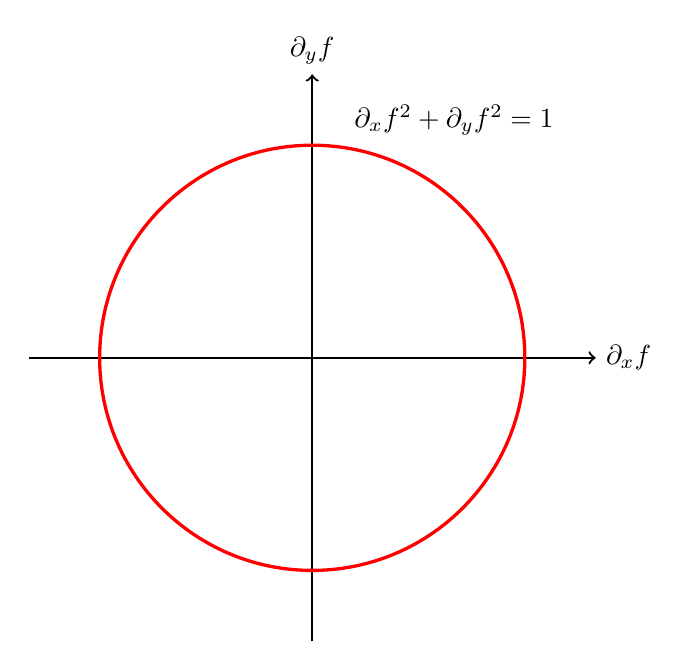
\begin{tikzpicture}[scale=0.9]
%\draw[help lines, color=gray!30, dashed] (-0.9,-0.9) grid (4.9,4.9);
\draw[->, thick] (-4,0)--(4,0) node[right]{$\partial_x f$};
\draw[->, thick] (0,-4)--(0,4) node[above]{$\partial_y f$};
\draw[color=red, very thick](0,0) circle (3);
\node[above] at (2,3) {$\partial_xf^2+\partial_yf^2=1$};
\end{tikzpicture}
\end{subfigure}
\caption{The constraint manifold $\mathcal{M}_\mathcal{C}=\{\partial_xf^2+\partial_yf^2=1\}$ in the space of first order derivatives $(\partial_x f,\partial_yf)$.}
\end{figure}



%%%%%%%%%%%%%%%%%%%%%%%%%%%%%%%%%%%%%%%%%%%%%%%%%%%%%%%%%%%%%%%%
\section{Constraint initial conditions of the caustic skeleton}
Given non-linear constrained Gaussian random field theory and the caustic conditions, we study the progenitors of the filaments and clusters in the Zel'dovich approximation. Given the displacement field 
\begin{align}
\bm{s}_t(\bm{q}) = -b_+(t) \nabla_{\bm{q}} \Psi(\bm{q}),
\end{align}
it is convenient to express the deformation tensor
\begin{align}
\bm{\psi}(\bm{q}) = \begin{pmatrix} T_{11}(\bm{q}) & T_{12}(\bm{q}) \\ T_{12}(\bm{q}) & T_{22}(\bm{q})\end{pmatrix}
\end{align}
in terms of the partial derivatives of the displacement potential $T_{ij\dots k}=\frac{\partial}{\partial q_i}\frac{\partial}{\partial q_j}\dots \frac{\partial}{\partial q_k}\Psi$. The eigenvalue and eigenvector fields of $\bm{\psi}$ defined by
\begin{align}
\bm{\psi}(\bm{q}) \bm{v}_i(\bm{q}) = \lambda_i(\bm{q}) \bm{v}_i(\bm{q}),
\end{align}
with the ordering $\lambda_1\geq \lambda_2$. We normalize the eigenvector field to unity, \textit{i.e.}, $\|\bm{v}_{i}\|=1$. We can express the eigenvalue and eigenvector fields explicitly in terms of the second order derivatives of the deformation potential
\begin{align}
\lambda_{1,2} &= \frac{1}{2}\left[T_{11}+T_{22} \pm \sqrt{4 T_{12}^2+(T_{11}-T_{22})^2}\right]\,,\\
\bm{v}_{1,2} &\propto \left(T_{11}-T_{22} \pm \sqrt{4 T_{12}^2+(T_{11}-T_{22})^2}, 2 T_{12}\right)\,,
\end{align}
showing their non-linear dependence on the deformation potential. In the study below, we assume a power-law power spectrum for the gravitational potential
\begin{align}
P(k)=k^{-1}
\end{align}
with a Gaussian smoothing at a scale $\sigma = 5 \text{ Mpc}$.

%%%%%%%%%%%%%%%%%%%%%%%%%%%%%%%%%%%%%%%%%%%%%%%%%%%%%%%%%%%%%%%%
\subsection{Cusp filament}
A cusp caustic forming at time $t$ corresponding to the largest eigenvalue field $\lambda_1$ satisfies the conditions
\begin{align}
b_+(t) \lambda_1(\bm{q}) = 1\,, \quad \bm{v}_1(\bm{q}) \cdot \nabla\lambda_1(\bm{q}) = 0\,.
\end{align}
The orientation of the cusp is determined by the normal vector
\begin{align}
\bm{n} =  \nabla(\bm{v}_1(\bm{q}) \cdot \nabla\lambda_1(\bm{q}))\,.
\end{align}
In the eigenframe, for which $\bm{v}_1=(1,0)$ and $\bm{v}_2=(0,1)$, these conditions simplify to a set of linear conditions on the second and third order derivatives of the deformation potential
\begin{align}
T_{11}=1/b_+(t)\,, \quad T_{12}=0\,,\quad T_{22}\leq T_{11}\,,\quad T_{111}=0\,.
\end{align}
The normal vector yields the non-linear form
\begin{align}
\bm{n}=\left(T_{1111} + \frac{3T_{112}^2}{T_{11}-T_{22}}, T_{1112} + \frac{3T_{112}T_{122}}{T_{11}-T_{22}}\right)\,.
\end{align}
More specifically, the normal vector makes an angle $\alpha = \text{sign}(\bm{v}_2\cdot \bm{n}) \arccos\left(|\bm{v}_1\cdot \bm{n}|/ \|\bm{n}\|\right)$ with respect to the eigenvector $\bm{v}_1$.

Let's first consider the configuration of a cusp curve going through the origin of the box while ignoring the orientation of the line. The cusp caustic in the eigenvector frame is fully determined by the derivatives $Y=(T_{11},T_{12},T_{22},T_{111})$, whose probability density factorizes into the density of the joint distribution of $T_{11}$ and $T_{22}$ and the one-dimensional Gaussian distributions for $T_{12}$ and $T_{111}$, \textit{i.e.},
\begin{align}
p(T_{11},T_{12},T_{22},T_{111}) = p(T_{11},T_{22})p(T_{12})p(T_{111}).
\end{align}
The conditional density corresponding to the cusp conditions reduces to the conditional probability density of $T_{22}$ given $T_{11}$, \textit{i.e.},
\begin{align}
p&(T_{11},T_{12},T_{22},T_{111}|,T_{22}\leq T_{11}=1/b_+,T_{12}=0,T_{111}=0) \\
&= p(T_{22}| T_{22} \leq T_{11}=1/b_+)\\
&= \mathcal{N} e^{-\frac{3(T_{11} + T_{22})^2 - 8 T_{11} T_{22}}{2 \sigma_2^2}}\big|_{T_{11}=1/b_+}
\end{align}
with the normalization constant $\mathcal{N}$. After sampling $T_{22}$ from this distribution, we can use linear constrained random field theory to obtain the corresponding realization. Note that this is equivalent to generating realizations for the linear constraints $T_{11}=1/b_+,T_{12}=T_{111}=0$ and rejecting realizations for which $T_{22} > 1/b_+$. The mean field is determined by the expectation value $\langle T_{22} \rangle$. The variance is fully determined by the variables $T_{11},T_{12},T_{22},T_{111}$.

The orientation of the cusp curve is fully characterized by the derivatives  
\begin{align}
Y=(T_{11},T_{12},T_{22},T_{111},T_{112},T_{122},T_{1111},T_{1112})
\end{align}
with the conditional distribution
\begin{align}
&p(T_{11},T_{12},T_{22},T_{111},T_{112},T_{122},T_{1111},T_{1112}|T_{22} \leq T_{11}=1/b_+, T_{111}=0)\\
&=
p(T_{11},T_{22},T_{1111}|T_{22}\leq T_{11}=1/b_+)p(T_{12}T_{1112}|T_{12}=0)p(T_{111},T_{122}|T_{111}=0)p(T_{112})\,.
\end{align}
Alternatively, we can sample from this distribution using the constraint realizations described above. The distribution for $\alpha$ is centred around $\alpha=0$, \textit{i.e.}, the cusp curve is biased to be normal to the eigenvector field $\bm{v}_1$ (see figure \ref{fig:alpha}).

\begin{figure}
\centering
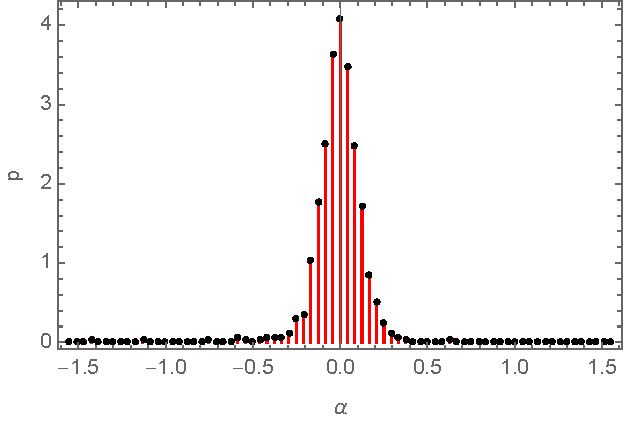
\includegraphics[width=0.5\textwidth]{alpha}
\caption{The distribution of the angle $\alpha$} 
\label{fig:alpha}
\end{figure}

There are two ways in which we can fix the orientation of the cusp curve in the constraint realizations. Firstly, note that the orientation of the cusp curve is fully determined by the second, third, and fourth order derivatives of the deformation potential. For the first method, we sample the second, third, and fourth order derivatives from the conditional distribution with the conditions that $b_+\lambda_1=1, \bm{v}_1 \cdot \nabla \lambda = 0$ and $\bm{n}\cdot (0,1) = 0$. Given this sample, we can use linear constraint theory to find the realization. However, by fixing the orientation of the normal $\bm{n}$ we lose the freedom to rotate to the eigenframe $\bm{v}_1=(1,0), \bm{v}_2=(0,1)$ of the deformation tensor, making such a calculation difficult to execute. Alternatively, we can start with a realization of the cusp curve without the required orientation in the eigenframe and compute the corresponding second, third, and fourth order derivatives. Given the derivatives of the realization we evaluate the angle $\alpha$ and rotate these derivatives to the configuration for which the cusp curve is vertical in the origin (see appendix \ref{ap:rotations}). We can use these rotated derivatives to generate a realization for which the cusp curve passes vertically through the origin. By sampling the second, third, and fourth order derivatives of the rotated configuration, we can evaluate the mean field and the variance of the oriented cusp curve (see figure \ref{fig:meanCusp}).

We see that the cusp caustic caustic is an elongated blob. The presence of a cusp curve significantly influences its environment up to about a radius of $20\text{ Mpc}$ on a smoothing scale of $\sigma = 5 \text{ Mpc}$.


\begin{figure}
\centering
\begin{subfigure}[b]{0.32\textwidth}
\includegraphics[width=\textwidth]{Cusp_mean}
\caption{$\text{mean}(\Psi)$}
\end{subfigure}~
\begin{subfigure}[b]{0.32\textwidth}
\includegraphics[width=\textwidth]{Cusp_variance}
\caption{$\text{variance}(\Psi)$}
\end{subfigure}~
\begin{subfigure}[b]{0.32\textwidth}
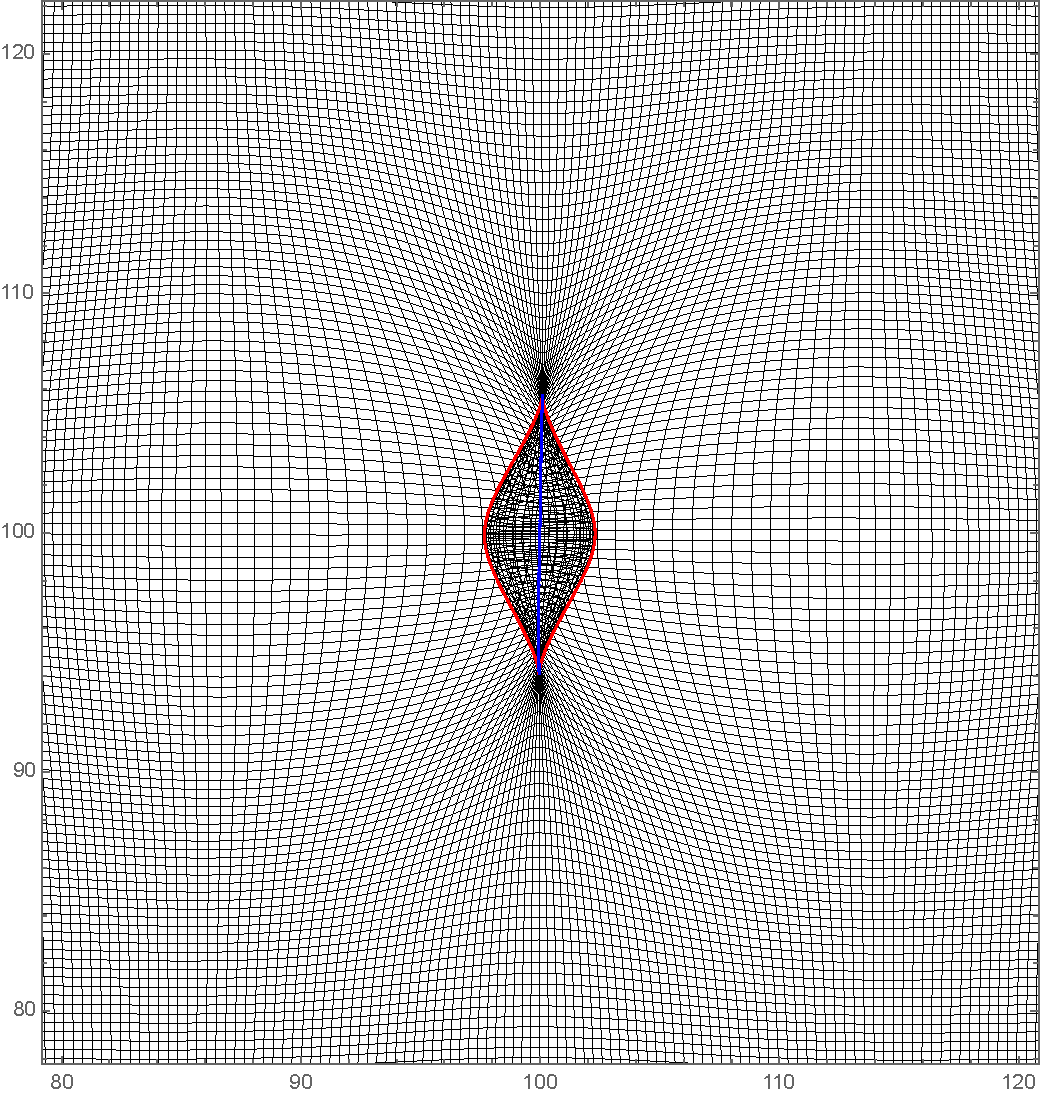
\includegraphics[width=\textwidth]{Cusp_E_Mean}
\caption{Zel'dovich}
\end{subfigure}
\caption{The mean and variance field of the cusp filament}\label{fig:meanCusp}
\end{figure}




\begin{figure}
\centering
\begin{subfigure}[b]{0.32\textwidth}
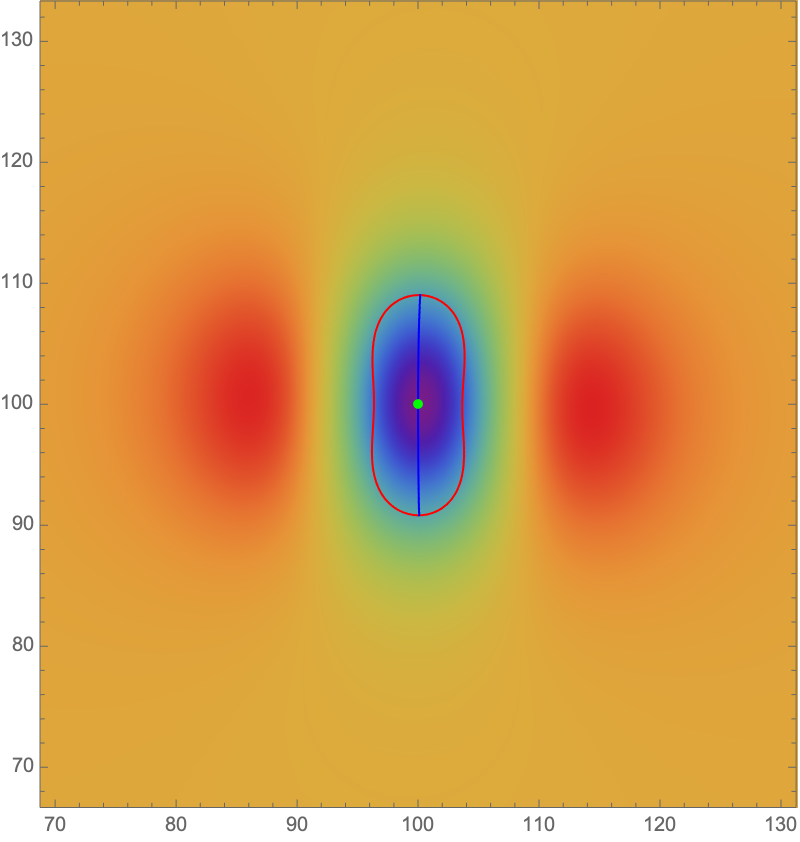
\includegraphics[width=\textwidth]{Cusp_mean_Phi}
\end{subfigure}~
\begin{subfigure}[b]{0.32\textwidth}
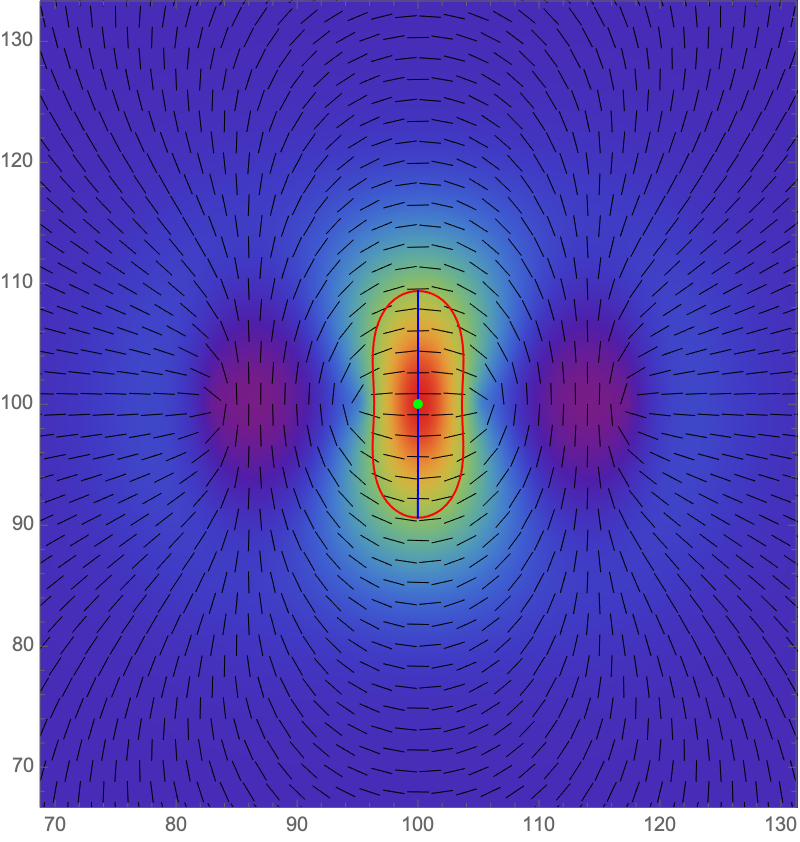
\includegraphics[width=\textwidth]{Cusp_mean_L}
\end{subfigure}~
\begin{subfigure}[b]{0.32\textwidth}
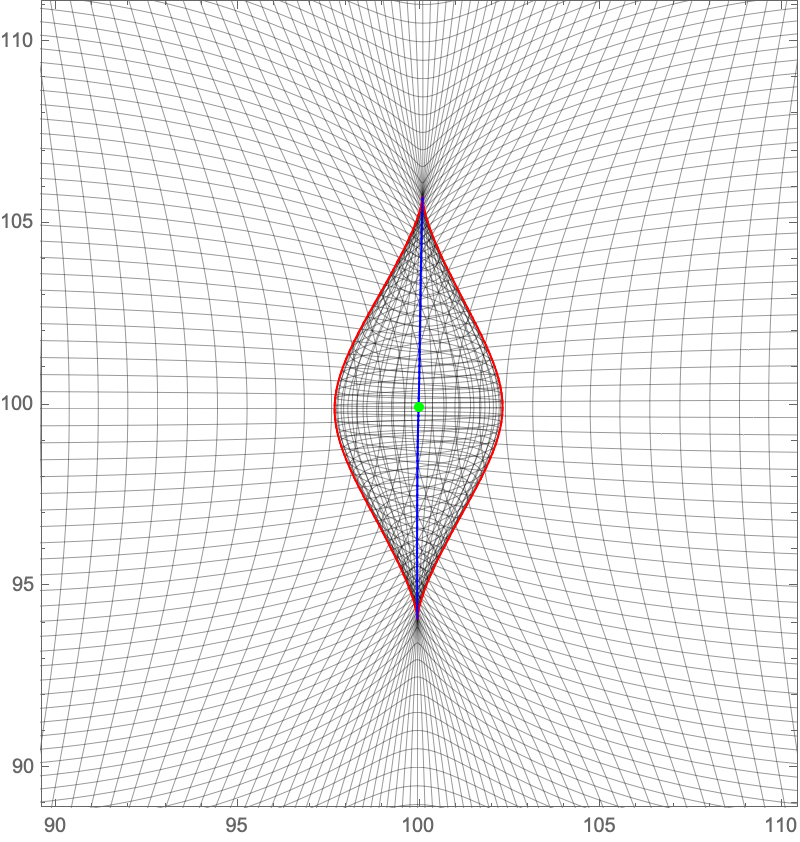
\includegraphics[width=\textwidth]{Cusp_mean_Z}
\end{subfigure}
\caption{The mean cusp caustic. \text{Left:} the gravitational potential. \textit{Centre:} the first eigenvalue and eigenvector fields. \textit{Right:} The Zel'dovich approximation}\label{fig:meanCusp}
\end{figure}

%%%%%%%%%%%%%%%%%%%%%%%%%%%%%%%%%%%%%%%%%%%%%%%%%%%%%%%%%%%%%%%%
\subsection{Swallowtail cluster}
The swallowtail caustic is determined by the conditions
\begin{align}
b_+(t) \lambda_1(\bm{q}) = 1\,, \quad \bm{v}_1(\bm{q}) \cdot \nabla_{\bm{q}}\lambda_1(\bm{q}) = 0\,, \quad\bm{v}_1\cdot \nabla_{\bm{q}}( \bm{v}_1(\bm{q}) \cdot \nabla_{\bm{q}}\lambda_1(\bm{q})) = 0\,.
\end{align}
In the eigenframe, the caustic conditions for the cusp take the form
\begin{align}
T_{11}=1/b_+(t)\,, \quad T_{12}=0\,,\quad T_{22}\leq T_{11}\,,\quad T_{111}=0\,, \quad T_{1111}+\frac{3T_{112}^2}{T_{11}-T_{22}} =0\,.
\end{align}
The cusp curve in the swallowtail caustic is parallel to the eigenvector field $\bm{v}_1$ since $\bm{v}_1 \cdot \bm{n}=0$ or $\alpha = \pm \pi/2$. Hence, the swallowtail caustic does not require us to fix its orientation.

The swallowtail caustic is determined by the variables $Y=(T_{11},T_{12},T_{22},T_{111},T_{112},T_{1111})$ with the probability density
\begin{align}
p(T_{11},T_{12},T_{22},T_{111},T_{112},T_{1111})=p(T_{11},T_{22},T_{1111})p(T_{12})p(T_{111})p(T_{112})\,.
\end{align}
The constraint distribution takes the form
\begin{align}
&p\left(T_{22},T_{112},T_{1111}|T_{22}\leq T_{11}=1/b_+, T_{12}=0,T_{111}=0,T_{1111}+\frac{3T_{112}^2}{T_{11}-T_{22}}=0\right)\\
=&\, p\left(T_{22},T_{112}, T_{1111}|T_{22}\leq T_{11}=1/b_+, T_{1111}+\frac{3T_{112}^2}{T_{11}-T_{22}}=0\right)\,.
\end{align}
The first condition can be straightforwardly implemented using the discussion for the cusp curve. The second condition is more subtle due to its non-linear nature. However, there exists an efficient method using rejection sampling based on the independence of the variable $T_{112}$ in the joint distribution.

Firstly, consider the conditional distribution
\begin{align}
p(T_{22},T_{1111}|T_{11}=1/b_+)\,.
\end{align}
Since the joint distribution $p(T_{11},T_{22},T_{1111})$ is Gaussian with vanishing mean $\bm{\mu}=\bm{0}$, and the covariance matrix $\begin{pmatrix} a & \bm{b} \\ \bm{b}^T & \Sigma \end{pmatrix}$, the constraint distribution $p(T_{22},T_{1111}|T_{11}=1/b_+)$, with $a=5 \sigma_3^2/16$, is agian a multidimensional Gaussian distribution, with mean $\bar{\bm{\mu}}=\frac{\bm{b}}{a b_+}$ and the covariance matrix $\bar{\Sigma}=\Sigma -\frac{1}{a} \bm{b}\bm{b}^T$. After sampling from this distribution, we can reject realizations for which $T_{22}>1/b_+$ or $T_{1111}>0$ to obtain samples from the auxiliary probability density $p(T_{22},T_{1111}| T_{22} \leq T_{11}=1/b_+,T_{1111}\leq 0)$. Finally, note that the non-linear condition fully determines $T_{112}^2$ in terms of $T_{11},T_{22},T_{1111}$ when $T_{22} < T_{11}$ and $T_{1111}\leq 0$. The variable $T_{112}$ in the joint distribution is an independent Gaussian variable with zero mean $\langle T_{112}\rangle = 0$ and variance $\langle T_{112}^2\rangle = \sigma_3^2/16$. We can thus write the unnormalized density of the conditional density as a product of the conditional density $p(T_{22},T_{1111}|T_{22}\leq T_{11}=1/b_+,T_{1111})$ and a function between $0$ and $1$,
\begin{align}
p(T_{22},T_{1111}) \propto e^{-\frac{1}{2}((T_{22},T_{1111})-\bar{\bm{\mu}})\bar{\Sigma}^{-1}((T_{22},T_{1111})-\bar{\bm{\mu}}) }\Theta(1/b_+-T_{22})\Theta(-T_{1111})e^{ \frac{8T_{1111} (1/b_+ - T_{22})}{3 \sigma_3^2}}
\end{align}
with the Heaviside step function $\Theta$. We can thus obtain realizations of the target conditional density by sampling from the distribution $p(T_{22},T_{1111}|T_{22}\leq T_{11}=1/b_+,T_{1111})$ and accepting the realization with probability $\exp\left[ \frac{8T_{1111} (1/b_+ - T_{22})}{3 \sigma_3^2}\right]$. The mean and variance fields can be evaluating the expectation values of the second, third, and fourth order derivatives of the deformation potential (see figure \ref{fig:meanSwallowtail}).



\begin{figure}
\centering
\begin{subfigure}[b]{0.32\textwidth}
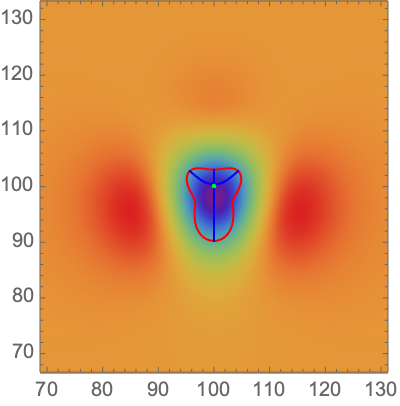
\includegraphics[width=\textwidth]{Swallowtail_mean_Phi}
\end{subfigure}~
\begin{subfigure}[b]{0.32\textwidth}
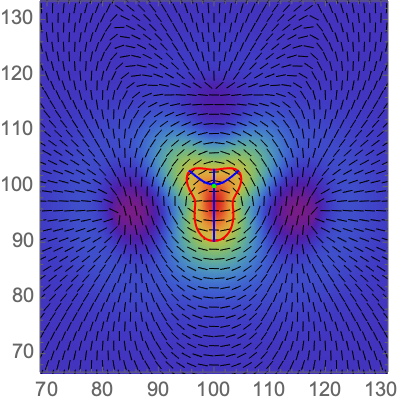
\includegraphics[width=\textwidth]{Swallowtail_mean_L}
\end{subfigure}~
\begin{subfigure}[b]{0.32\textwidth}
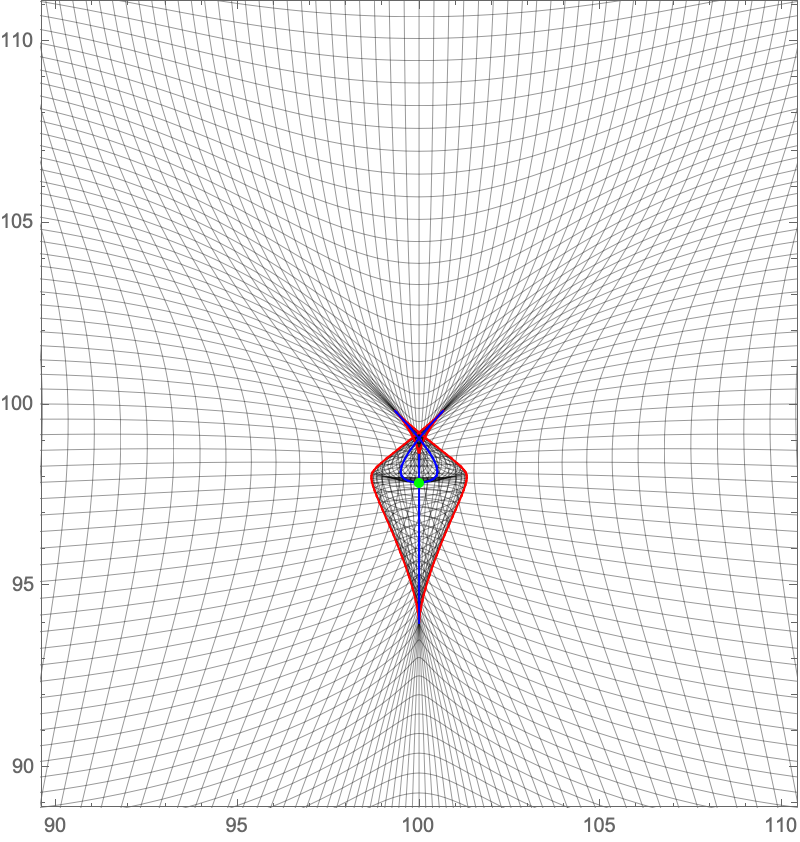
\includegraphics[width=\textwidth]{Swallowtail_mean_Z}
\end{subfigure}
\caption{The mean swallowtail caustic. \text{Left:} the gravitational potential. \textit{Centre:} the first eigenvalue and eigenvector fields. \textit{Right:} The Zel'dovich approximation}\label{fig:meanSwallowtail}
\end{figure}

%%%%%%%%%%%%%%%%%%%%%%%%%%%%%%%%%%%%%%%%%%%%%%%%%%%%%%%%%%%%%%%%
\subsection{Umbilic cluster}
The umbilic caustics form when $\lambda_1(\bm{q}) = \lambda_2(\bm{q}) = 1/b_+(t)$, corresponding to the linear conditions
\begin{align}
T_{11}=T_{22}=1/b_+(t)\,, \quad T_{12}=0\,.
\end{align}
In the umbilic caustic, the determinant 
\begin{align}
\det (I- b_+ \bm{\psi})
\end{align}
is a critical point. The nature of the critical point is determined by the Hessian
\begin{align}
\mathcal{H}\left[\det (I- b_+ \bm{\psi})\right] =
\begin{pmatrix} 
2(T_{111}T_{122} -T_{112}^2) & T_{111}T_{222}-T_{112}T_{122} \\
T_{111}T_{222}-T_{112}T_{122} & 2(T_{112}T_{222}-T_{122}^2)
\end{pmatrix}\,.
\end{align}
Note that the Hessian is fully determined by the third order derivatives of the deformation potential. When the critical point is a maximum, or a minimum, \textit{i.e.},
\begin{align}
\det (\mathcal{H}\left[\det (I- b_+ \bm{\psi})\right]) >0\,,
\end{align}
the umbilic caustic is an elliptic caustic. When the critical point is a saddle point, \textit{i.e.},
\begin{align}
\det (\mathcal{H}\left[\det (I- b_+ \bm{\psi})\right]) <0\,,
\end{align}
the umbilic caustic is a hyperbolic caustic. The easiest way to obtain realizations of these umbilic caustics is to implement the linear constraints and determine the determinant is positive or negative.

The orientation of the elliptic umbilic caustic is determined by the behaviour of the eigenvector fields of the deformation tensor in the vicinity of the caustic. The fold curve in the vicinity of the elliptic umbilic caustic is a small circle, which forms three cusp caustics when the eigenvector field is parallel to the eigenvector field, $\bm{v}_i \cdot \bm{m} = 0$ with $\bm{m}$ the vector normal to this circle.

The orientation and configuration of the hyperbolic umbilic caustic is determined by the eigenvalues $\lambda_i$ and eigenvectors $\bm{w}_i$ of the Hessian $\mathcal{H}\left[\det (I- b_+ \bm{\psi})\right]$. The cusp curve of the hyperbolic umbilic is directed towards the eigenvector corresponding to the positive eigenvalue field. We can fix the orientation by implementing the conditions
\begin{align}
T_{111}T_{222}-T_{112}T_{122}&=0\,,\\
T_{111}T_{122} -T_{112}^2 &\geq T_{112}T_{222}-2T_{122}^2\,.
\end{align}
However, it is easier to evaluate the eigenvector numerically for a realization and rotate the second and third order derivatives of the deformation tensor to obtain the required orientation (see appendix \ref{ap:rotations}). The angle of the wedge of the fold curve is determined by the ratio of the eigenvalues $\beta = 2 \arctan(\sqrt{|\nu_1/\nu_2|})$.

\begin{figure}
\centering
\begin{subfigure}[b]{0.32\textwidth}
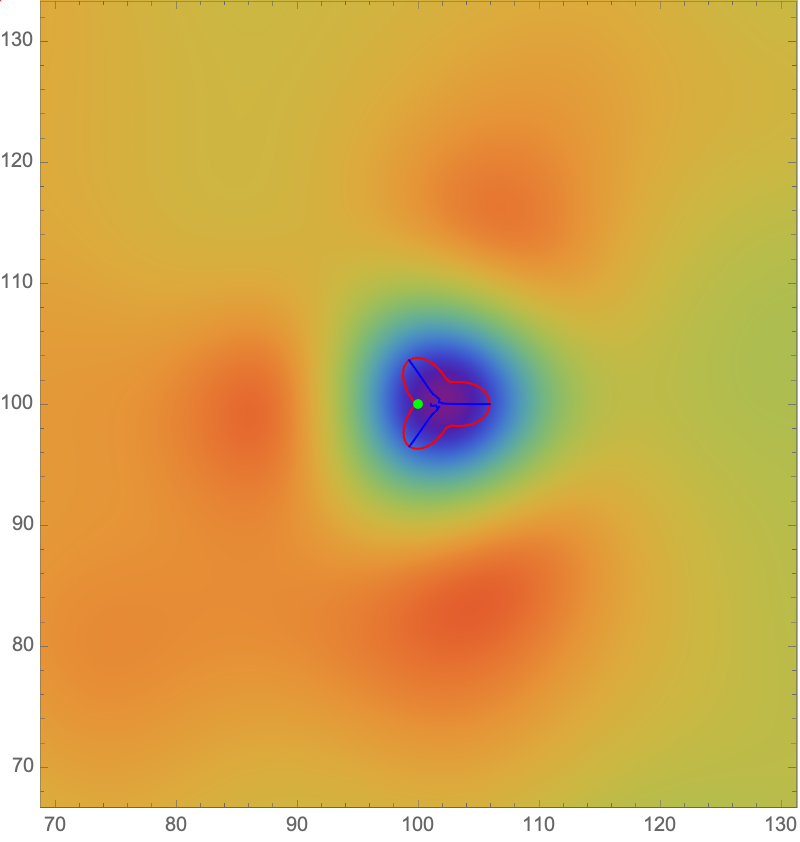
\includegraphics[width=\textwidth]{Hyperbollic_mean_Phi}
\end{subfigure}~
\begin{subfigure}[b]{0.32\textwidth}
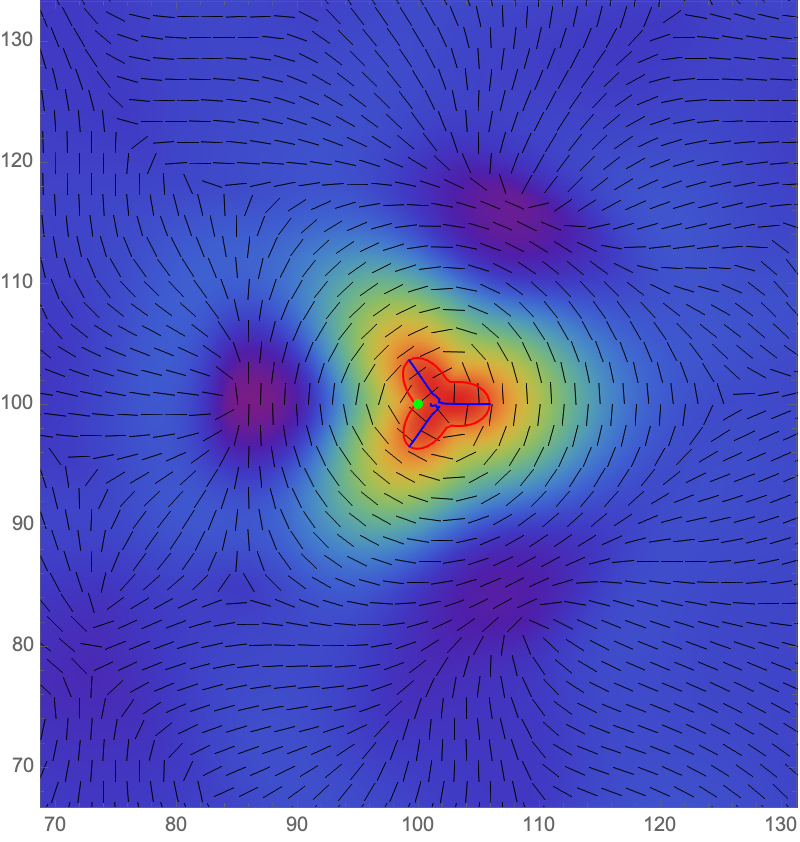
\includegraphics[width=\textwidth]{Hyperbollic_mean_L}
\end{subfigure}~
\begin{subfigure}[b]{0.32\textwidth}
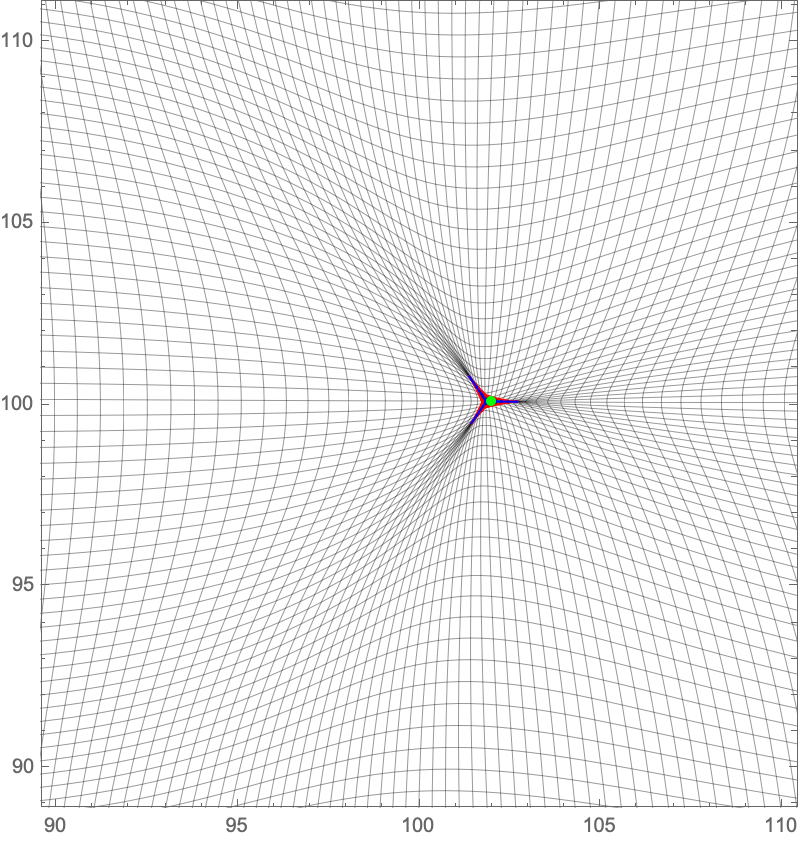
\includegraphics[width=\textwidth]{Hyperbollic_mean_Z}
\end{subfigure}
\caption{The mean hyperbollic caustic. \text{Left:} the gravitational potential. \textit{Centre:} the first eigenvalue and eigenvector fields. \textit{Right:} The Zel'dovich approximation}\label{fig:meanSwallowtail}
\end{figure}


%%%%%%%%%%%%%%%%%%%%%%%%%%%%%%%%%%%%%%%%%%%%%%%%%%%%%%%%%%%%%%%%
\section{Composite constraint realizations}
In practice, we wish to constrained realizations with several constraints corresponding to caustics with specific orientations. First let's consider the ways in which we can vary the orientation of a caustic. In the previous section, we studied how we can construct a realization with a cusp filament running vertically through the origin of the simulation. Note that the cusp curve and its orientation is fully determined by the seccond, third, and fourth order derivatives of the gravitational potential in the caustic. Now, given a realiation of a unconstrained Gaussian random field, we generate a constrained realization with a vertically oriented cusp curve. For this realization, we evaluate the second, third, and fourth order derivatives in the caustic. Using appendix \ref{ap:rotations}, we can obtain a rotated set of constrained conditions corresponding to a cusp curve whose tangent vector makes an angle $\theta$ with the vertical axis in the origin. By generating a corresponding constrained realization, we can rotate the cusp curve to any orientation. In figure \ref{fig:rotation}, we rotate the cusp filament while reusing the unconstraint Gaussian random field.

\begin{figure}
\centering
\begin{subfigure}[b]{0.31\textwidth}
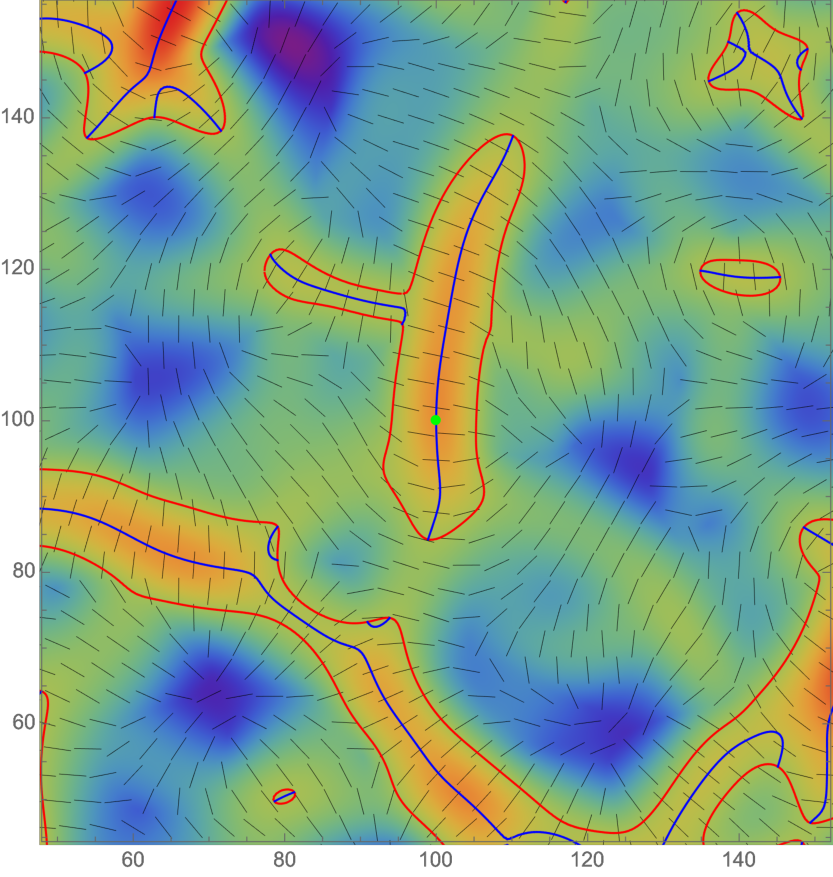
\includegraphics[width=\textwidth]{Rotation_L_1}
\end{subfigure}~
\begin{subfigure}[b]{0.31\textwidth}
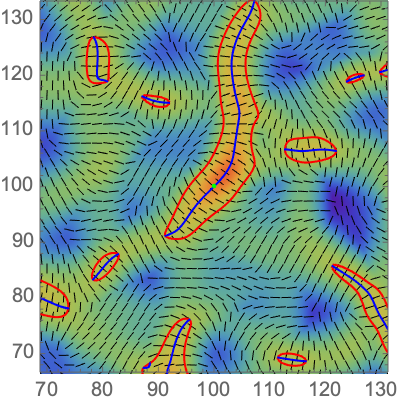
\includegraphics[width=\textwidth]{Rotation_L_2}
\end{subfigure}~
\begin{subfigure}[b]{0.31\textwidth}
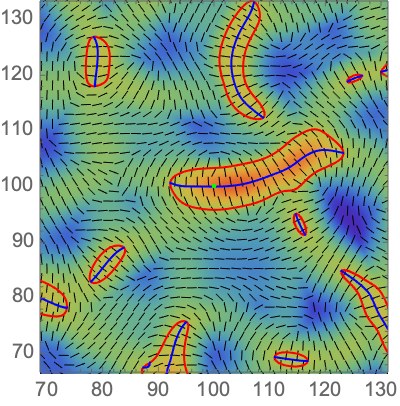
\includegraphics[width=\textwidth]{Rotation_L_3}
\end{subfigure}\\
\begin{subfigure}[b]{0.31\textwidth}
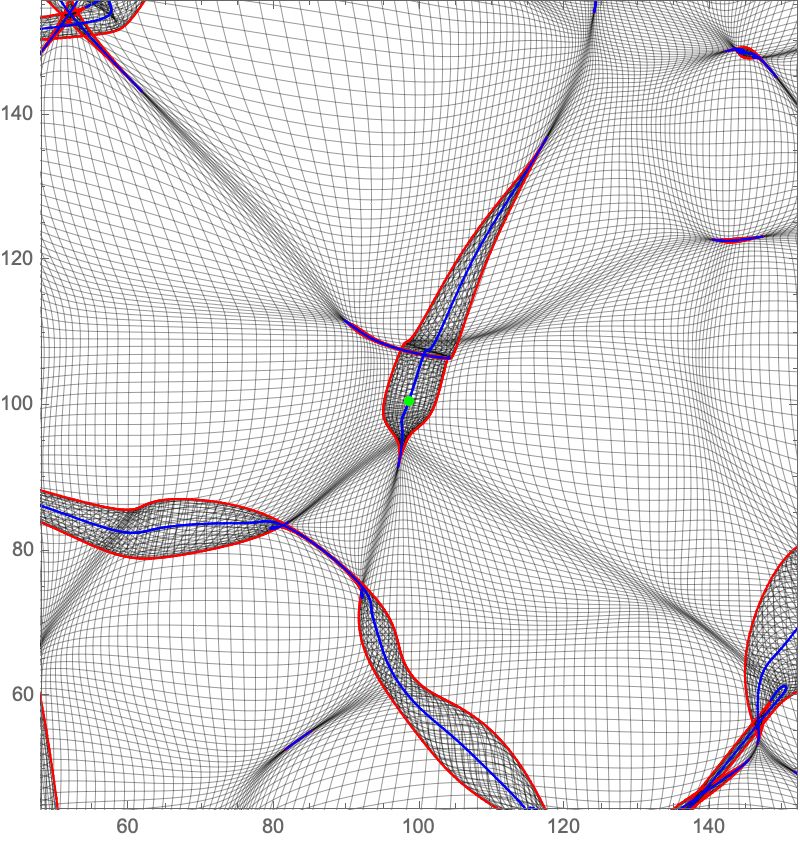
\includegraphics[width=\textwidth]{Rotation_Z_1}
\end{subfigure}~
\begin{subfigure}[b]{0.31\textwidth}
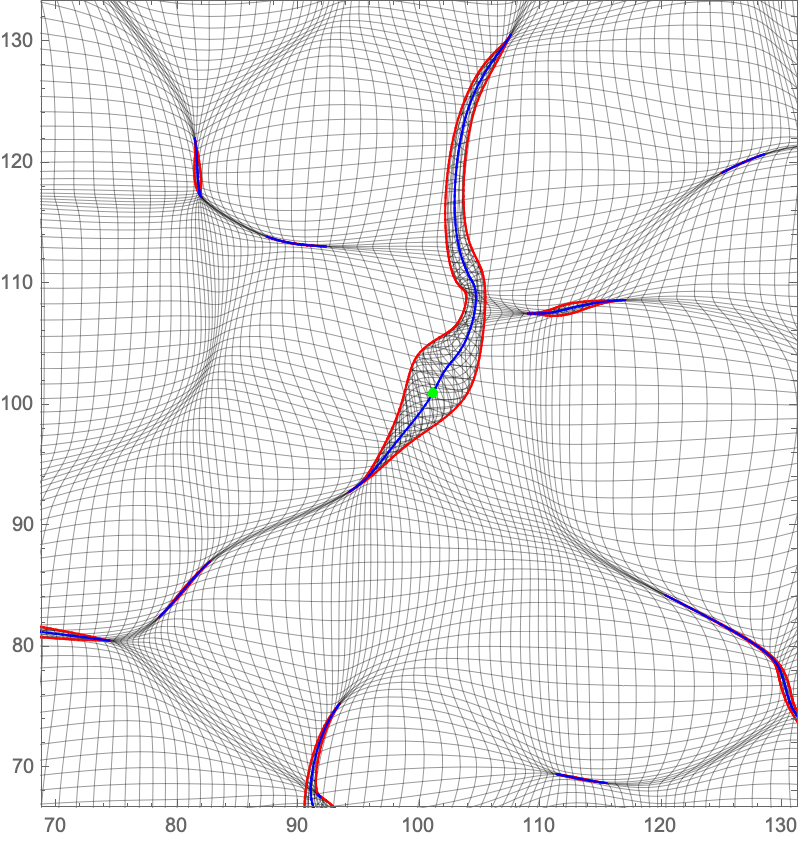
\includegraphics[width=\textwidth]{Rotation_Z_2}
\end{subfigure}~
\begin{subfigure}[b]{0.31\textwidth}
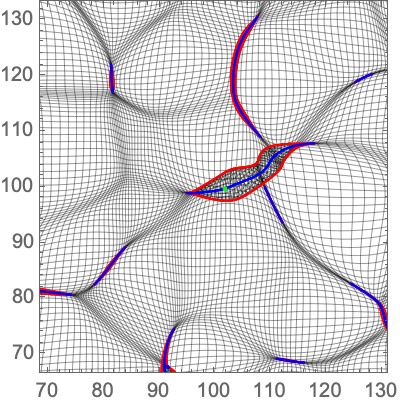
\includegraphics[width=\textwidth]{Rotation_Z_3}
\end{subfigure}
\caption{Rotation of the cusp caustic. \textit{Upper:} the eigenvalue and eigenvector fields in Lagrangian space. \textit{Lower:} the Zel'dovich approximation in Eulerian space. \textit{Left:} with the vertical orientation. \textit{Center:} with a diagonal orientation. \textit{Right:} with the horizontal orientation.}\label{fig:rotation}
%%%%%%%%%%%%%%%5
\centering
\begin{subfigure}[b]{0.46\textwidth}
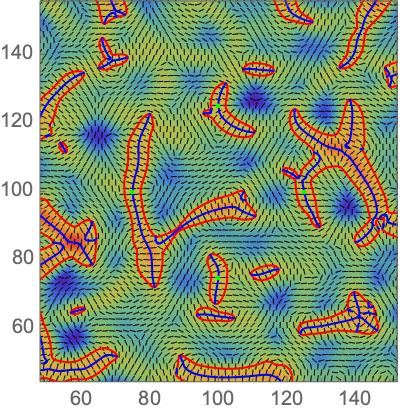
\includegraphics[width=\textwidth]{Composite_L}
\end{subfigure}~
\begin{subfigure}[b]{0.46\textwidth}
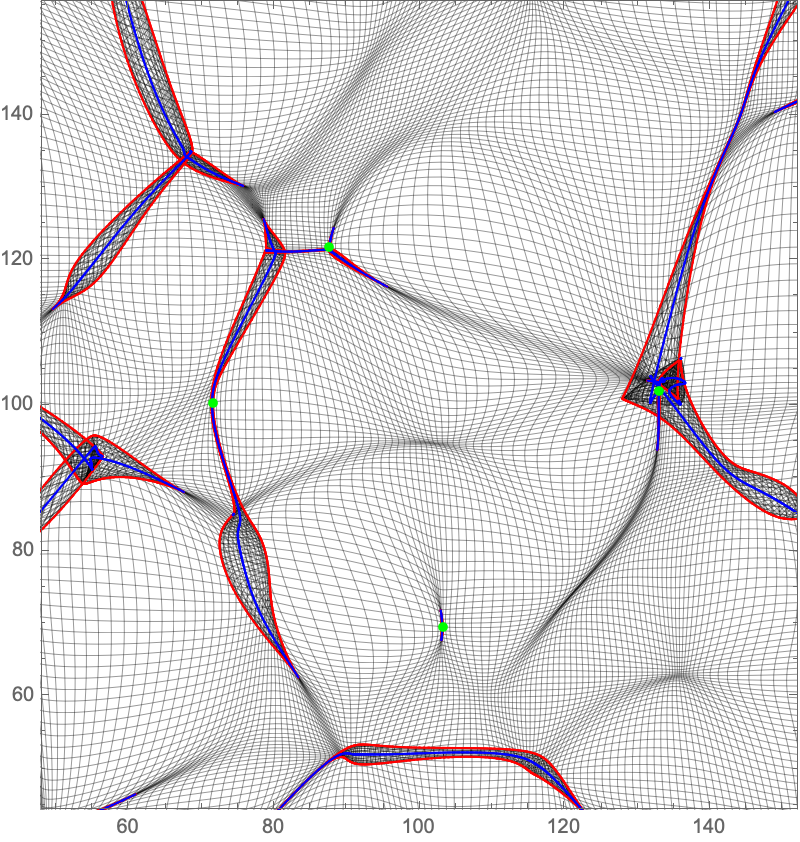
\includegraphics[width=\textwidth]{Composite_Z}
\end{subfigure}
\caption{Four critical point constraints on the first eigenvalue field. \textit{Left:} the first eigenvalue and eigenvector fields in Lagrangian space. \textit{Right:} the Zel'dovich approximation in Eulerian space.}\label{fig:composite}
\end{figure}

Non-linear constrained theory also extends to a set of non-linear constraints. For example, consider a set of critical points of the first eigenvalue field. At such a critical point, 
\begin{align}
\nabla \lambda_1(\bm{q}_c) = 0\,,
\end{align}
with function value $\lambda_1(\bm{q}_c)=1/b_+$. In the eigenvector frame, this condition reduces to the linear constraints
\begin{align}
1/b_+ = T_{11} \geq T_{22}\,, \quad  T_{12}=0\,,\quad T_{111}=T_{112}=0\,.
\end{align}
The critical point is either a maximum, minimum corresponding to the Morse point $A_3^+$ or a saddle point corresponding to the Morse point $A_3^-$. When the determinant of the Hessian $\mathcal{H}\lambda_1$ is positive/negative, it is a $A_3^+$/ $A_3^-$ point. Note that in the eigenframe field, the Hessian takes the form
\begin{align}
\mathcal{H}\lambda_1 = 
\begin{pmatrix} 
T_{1111}+\frac{2T_{112}^2}{T_{11}-T_{22}} & T_{1112} + \frac{2 T_{112}T_{122}}{T_{11}-T_{22}} \\
T_{1112}+\frac{2 T_{112}T_{122}}{T_{11}-T_{22}} & T_{1122} + \frac{2 T_{122}^2}{T_{11}-T_{22}}
\end{pmatrix}\,.
\end{align}
See figure \ref{fig:composite} for an illustration of a realization with four eigenvalue critical point constraints. The lower, upper, and right critical points are maxima. The left critical point is a saddle point.




\newpage
%%%%%%%%%%%%%%%%%%%%%%%%%%%%%%%%%%%%%%%%%%%%%%%%%%%%%%%%%%%%%%%%
\section{The caustic skeleton in Eulerian space}








\newpage  
%%%%%%%%%%%%%%%%%%%%%%%%%%%%%%%%%%%%%%%%%%%%%%%%%%%%%%%%%%%%%%%%
\section{Conclusion and Discussion}



\newpage
\appendix

%%%%%%%%%%%%%%%%%%%%%%%%%%%%%%%%%%%%%%%%%%%%%%%%%%%%%%%%%%%%%%%%
\section{Non-linear eigenvalue relations}\label{ap:eigenvalueRel}
To evaluate the statistical properties of the caustics we will use shorthand for the derivatives of the displacement potential $T_{ijk\dots} = \frac{\partial}{\partial q_i}\frac{\partial}{\partial q_j}\frac{\partial}{\partial q_k}\dots \Psi$. In this notation, the deformation tensor takes the form
\begin{align}
\bm{\psi} = \begin{pmatrix} T_{11} & T_{12} \\ T_{12} & T_{22}\end{pmatrix}.
\end{align}

Under a rotation $\omega$, 
\begin{align}
(q_1,q_2) \mapsto  (q_1\cos \omega - q_2 \sin \omega, q_1 \sin \omega + q_2 \cos \omega)\,,
\end{align}
the deformation tensor transform as the doubly periodic functions
\begin{align}
T_{11} &\mapsto T_{11} \cos ^2 \omega  + T_{22} \sin^2 \omega  + T_{12}\sin 2\omega\,,\\
T_{12} &\mapsto \frac{1}{2}(T_{22}-T_{11})\sin 2 \omega + T_{12} \cos 2\omega\,,\\
T_{22} &\mapsto T_{11} \sin ^2 \omega  + T_{22} \cos^2 \omega  - T_{12} \sin 2\omega\,.
\end{align}
Note that there are two angles $\omega \in [0,\pi)$ for which the deformation tensor is in its eigenframe, \textit{i.e.}, $T_{12}=0$, one for which $T_{11}>T_{22}$ and one for which $T_{11}<T_{22}$, separated by an angle $\pi/2$. In this paper we will always use the eigenframe for which $T_{12}=0$ and $T_{11} \geq T_{22}$. In this frame, the eigenvalues and eigenvectors take the simple form 
\begin{align}
\lambda_{1} &= T_{11}\,,\quad \bm{v}_1=(1,0)\,,\\
\lambda_{2} &= T_{22}\,,\quad \bm{v}_2=(0,1)\,.
\end{align}
If we would impose the reverse condition $T_{11} \leq T_{22}$ the relations would flip.

Using the eigenvalue decomposition,
\begin{align}
\bm{\psi} = R^T \Lambda R\,,
\end{align}
with the diagonal matrix $\Lambda = \text{diag}(\lambda_1,\lambda_2)$ where $\lambda_1 \geq \lambda_2$ and the rotation matrix
\begin{align}
R = \begin{pmatrix} \cos \theta & - \sin \theta \\ \sin \theta & \cos \theta \end{pmatrix} \in SO(2),
\end{align}
we can express the components $T_{11},T_{22},T_{12}$ in terms of the eigenvalue coordinates $\lambda_1,\lambda_2,\theta$,
\begin{align}
T_{11} &= \lambda_1 \cos^2 \omega + \lambda_2 \sin^2 \theta\,,\\
T_{22} &= \lambda_1 \sin^2\omega + \lambda_2 \cos^2 \theta\,,\\
T_{12} &= (\lambda_2 - \lambda_1)\cos \theta \sin \theta\,.
\end{align}
Inverting this set of equation give the eigenvalues
\begin{align}
\lambda_1(T_{11},T_{22},T_{12}) &= \frac{1}{2}\left(T_{11}+T_{22} + \sqrt{4 T_{12}^2 +(T_{11}-T_{22})^2}\right)\,,\\
\lambda_2(T_{11},T_{22},T_{12}) &= \frac{1}{2}\left(T_{11}+T_{22} - \sqrt{4 T_{12}^2 +(T_{11}-T_{22})^2}\right)\,,
\end{align}
and the normalized eigenvector fields
\begin{align}
\bm{v}_1 &= (\cos(\theta), -\sin(\theta))\,,\\
\bm{v}_2 &= (\sin(\theta),\ \ \ \cos(\theta))\,,
\end{align}
with
\begin{align}
\cos(\theta) &= \frac{\sqrt{T_{11} - T_{22} + \sqrt{4 T_{12}^2 +(T_{11}-T_{22})^2}}}{\sqrt{2} \sqrt[4]{4T_{12}^2 + (T_{11}-T_{22})^2}}\,,\\
\sin(\theta) &= \frac{\sqrt{2}T_{12}}{\sqrt[4]{4T_{12}^2+(T_{11}-T_{22})^2}\sqrt{T_{11}-T_{22} + \sqrt{4T_{12}^2 + (T_{11}-T_{22})^2}}}\,.
\end{align}
Given the eigenvalue and eigenvector fields in terms of the second order derivatives of the displacement potential, we can evaluate the directional derivatives of the eigenvalue fields in the eigenframe $T_{12}=0, T_{11} \geq T_{22}$.

The first and second order derivatives of the eigenvalue fields in the eigenvector frame take the form
\begin{align}
\frac{\partial}{\partial q_1} \lambda_1&= T_{111}\,,\quad
\frac{\partial}{\partial q_2} \lambda_1= T_{112}\,,\\
\frac{\partial}{\partial q_1} \lambda_2&= T_{122}\,,\quad
\frac{\partial}{\partial q_2} \lambda_2= T_{222}\,,
\end{align}
and 
\begin{align}
\frac{\partial^2}{\partial q_1^2} \lambda_1&= T_{1111} + \frac{2 T_{112}^2}{T_{11}-T_{22}}\,,\\
\frac{\partial^2}{\partial q_1 \partial q_2} \lambda_1&= T_{1112} + \frac{2 T_{112}T_{122}}{T_{11}-T_{22}}\,,\\
\frac{\partial^2}{\partial q_2^2} \lambda_1&= T_{1122} + \frac{2T_{122}^2}{T_{11}-T_{22}}\,,\\
\frac{\partial^2}{\partial q_1^2} \lambda_2&= T_{1122} - \frac{2 T_{112}^2}{T_{11}-T_{22}}\,,\\
\frac{\partial^2}{\partial q_1 \partial q_2} \lambda_2&= T_{1222} - \frac{2 T_{112}T_{122}}{T_{11}-T_{22}}\,,\\
\frac{\partial^2}{\partial q_2^2} \lambda_2&= T_{2222} - \frac{2T_{122}^2}{T_{11}-T_{22}}\,.
\end{align}

These expressions differ from the directional derivatives in the eigenframe. The first order derivatives coincides with the gradient of the eigenvalue field
\begin{align}
\bm{v}_1 \cdot \nabla \lambda_1 &= T_{111}\,,\quad
\bm{v}_2 \cdot \nabla \lambda_1 = T_{112}\,,\\
\bm{v}_1 \cdot \nabla \lambda_2 &= T_{122}\,,\quad
\bm{v}_2 \cdot \nabla \lambda_2 = T_{222}\,.
\end{align}
The second order derivatives assume the form
\begin{align}
\bm{v}_1 \cdot \nabla (\bm{v}_1 \cdot \nabla \lambda_1) &= T_{1111} + \frac{3T_{112}^2}{T_{11}-T_{22}}\,,\\
\bm{v}_2 \cdot \nabla (\bm{v}_1 \cdot \nabla \lambda_1) &= T_{1112} + \frac{3T_{112}T_{122}}{T_{11}-T_{22}}\,,\\
\bm{v}_1 \cdot \nabla (\bm{v}_2 \cdot \nabla \lambda_1) &= T_{1112} - \frac{T_{112}(T_{111}-2T_{122})}{T_{11}-T_{22}}\,,\\
\bm{v}_2 \cdot \nabla (\bm{v}_2 \cdot \nabla \lambda_1) &= T_{1122} - \frac{T_{122}(T_{111}-2T_{122})}{T_{11}-T_{22}}\,,\\
\bm{v}_1 \cdot \nabla (\bm{v}_1 \cdot \nabla \lambda_2) &= T_{1122} + \frac{T_{112}(T_{222}-2T_{112})}{T_{11}-T_{22}}\,,\\
\bm{v}_2 \cdot \nabla (\bm{v}_1 \cdot \nabla \lambda_2) &= T_{1222} + \frac{T_{122}(T_{222}-2T_{112})}{T_{11}-T_{22}}\,,\\
\bm{v}_1 \cdot \nabla (\bm{v}_2 \cdot \nabla \lambda_2) &= T_{1222} - \frac{3T_{112}T_{122}}{T_{11}-T_{22}}\,,\\
\bm{v}_2 \cdot \nabla (\bm{v}_2 \cdot \nabla \lambda_2) &= T_{2222} - \frac{3T_{122}^2}{T_{11}-T_{22}}\,.
\end{align}

%%%%%%%%%%%%%%%%%%%%%%%%%%%%%%%%%%%%%%%%%%%%%%%%%%%%%%%%%%%%%%%%
\section{Constraint density}\label{ap:constraintDensity}
The conditional density 
\begin{align}
p(f|\Gamma) =\frac{p(f, \Gamma)}{p(\Gamma)}
\end{align}
with $\Gamma = \{\bm{C} = \bm{c}\}$ is a Gaussian density as both $p(f,\Gamma)$ and $p(\Gamma)$ are normally distributed. It thus suffices to evaluate the mean and covariance matrix. For completeness, we write the mean of the function and the constraints as $\bar{f}(\bm{q})=\langle f(\bm{q}) \rangle$ and $\bar{\bm{C}}=\langle \bm{C}\rangle$, and the covariance as
\begin{align}
\xi(\bm{q}_1,\bm{q}_2)& = \text{cov}(f(\bm{q}_1),f(\bm{q}_2))= \langle (f(\bm{q}_1) - \bar{f}(\bm{q}_1))(f(\bm{q}_2) - \bar{f}(\bm{q}_2))\rangle\,,\\
\xi_i(\bm{q}) &= \text{cov}(f(\bm{q}),C_i) = \langle (f(\bm{q})-\bar{f}(\bm{q}))(C_i - \bar{C}_i)\rangle\,,\\
\xi_{ij} &= \text{cov}(C_i,C_j) = \langle (C_i - \bar{C}_i)(C_j-\bar{C}_j)\rangle\,.
\end{align}
For conciseness, we will use the Einstein summation convention over the repeated dummy indices.

Define an auxiliary function $g(\bm{q}) = f(\bm{q}) + \bm{A}(\bm{q}) \cdot \bm{C}$ with $A_i(\bm{q}) = -\xi_i(\bm{q}) \xi_{ij}^{-1}$. The function $g$ is by construction independent of the variable $\bm{C}$, as they are jointly normally distributed and their covariance matrix vanishes, \textit{i.e.}, 
\begin{align}
\text{cov}(g(\bm{q}),\bm{C})
&=\text{cov}(f(\bm{q}),\bm{C}) +  \text{cov}(\bm{C},\bm{C}) \bm{A}(\bm{q}) \\
&=[\xi_k(\bm{q}) - \xi_i(\bm{q}) \xi_{ij}^{-1}\xi_{jk}]_{k=1}^N\\
&=\bm{0}\,.
\end{align}
The expectation value of $g$ is $\langle g(\bm{q})\rangle = \bar{f}(\bm{q}) + \bm{A}(\bm{q}) \cdot \bar{\bm{C}}$, which we can use to evaluate the expectation value of the constrained field
\begin{align}
\langle f(\bm{q}) | \Gamma \rangle 
&=\langle g(\bm{q}) - \bm{A}(\bm{q})\cdot \bm{C}|\Gamma\rangle\\
&=\langle g(\bm{q})\rangle - \bm{A}(\bm{q}) \cdot \bm{c}\\
&=\bar{f}(\bm{q}) + \bm{A}(\bm{q})\cdot (\bar{\bm{C}}-\bm{c})\\
&= \bar{f}(\bm{q}) + \xi_i(\bm{q})\xi_{ij}^{-1}(c_j -\bar{C}_j)\,.
\end{align}
When $\bar{f} = 0$ and $\bar{\bm{C}}=\bm{0}$ the expectation value reduces to the identity $\langle f(\bm{q}) | \Gamma \rangle =\xi_i(\bm{q})\xi_{ij}^{-1}c_j$. The covariance of the constraint field follows along similar lines
%\begin{align}
%\text{var}(f(\bm{q})|\Gamma) 
%&= \text{var}(g(\bm{q}) - \bm{A}(\bm{q})\cdot \bm{C}|\Gamma) \\
%&= \text{var}(g(\bm{q})|\Gamma) + \text{var}(\bm{A}(\bm{q})\cdot \bm{C}|\Gamma) -2 \bm{A}(\bm{q})\cdot \text{cov}(g(\bm{q}), \bm{C}|\Gamma)\\
%&= \text{var}(g(\bm{q})) \\
%&=\text{var}(f(\bm{q}) + \bm{A}(\bm{q})\cdot \bm{C})\\
%&=\text{var}(f(\bm{q})) + \bm{A}^T(\bm{q}) \text{var}(\bm{C}) \bm{A}(\bm{q}) + 2\bm{A}(\bm{q}) \cdot \text{cov}(f(\bm{q}),\bm{C}) \\
%&=\text{var}(f(\bm{q})) + \xi_i(\bm{q})\xi_{ij}^{-1}\xi_{jk}\xi_{kl}^{-1}\xi_{l}(\bm{q}) - 2\xi_i(\bm{q})\xi_{ij}^{-1}\xi_{j}(\bm{q})\\
%&=\xi(\bm{0}) - \xi_i(\bm{q}) \xi_{ij}^{-1} \xi_j(\bm{q})\,.
%\end{align}
\begin{align}
\text{cov}(f(\bm{q}_1), f(\bm{q}_2)|\Gamma) 
&= \text{cov}(g(\bm{q}_1) - \bm{A}(\bm{q}_1)\cdot \bm{C}, g(\bm{q}_2) - \bm{A}(\bm{q}_2)\cdot \bm{C}|\Gamma) \\
&= \text{cov}(g(\bm{q}_1), g(\bm{q}_2)|\Gamma) + \text{cov}(\bm{A}(\bm{q}_1)\cdot \bm{C}, \bm{A}(\bm{q}_2)\cdot \bm{C}|\Gamma)\\
&\ \ \  - \bm{A}(\bm{q}_1)\cdot \text{cov}(\bm{C}, g(\bm{q}_2)|\Gamma) -\text{cov}(g(\bm{q}_1) , \bm{C}|\Gamma)\cdot \bm{A}(\bm{q}_2)\\
&= \text{cov}(g(\bm{q}_1), g(\bm{q}_2)) \\
&=\text{cov}(f(\bm{q}_1) + \bm{A}(\bm{q}_1)\cdot \bm{C}, f(\bm{q}_2) + \bm{A}(\bm{q}_2)\cdot \bm{C})\\
&=\text{cov}(f(\bm{q}_1), f(\bm{q}_2)) + \bm{A}(\bm{q}_1) \text{cov}(\bm{C},\bm{C}) \bm{A}^T(\bm{q}_2) \\
&\ \ \ + \bm{A}(\bm{q}_1) \cdot \text{cov}(\bm{C},f(\bm{q}_2))+ \text{cov}(f(\bm{q}_1), \bm{C}) \cdot \bm{A}(\bm{q}_2) \\
&=\text{cov}(f(\bm{q}_1), f(\bm{q}_2)) + \xi_i(\bm{q}_1)\xi_{ij}^{-1}\xi_{jk}\xi_{kl}^{-1}\xi_{l}(\bm{q}_2) - 2\xi_i(\bm{q}_1)\xi_{ij}^{-1}\xi_{j}(\bm{q}_2)\\
&=\xi(\bm{q}_1,\bm{q}_2) - \xi_i(\bm{q}_1) \xi_{ij}^{-1} \xi_j(\bm{q}_2)\,.
\end{align}
We conclude that the residue $\delta f$ of $f$ with respect to the mean field $\langle f(\bm{q})|\Gamma\rangle =\bar{f}(\bm{q})+ \xi_i(\bm{q})\xi_{ij}^{-1}(c_j-\bar{C}_j)$ is a Gaussian random field with zero mean and variance $\sigma_0^2 - \xi_i(\bm{q}) \xi_{ij}^{-1} \xi_j(\bm{q})$. Note that the statistical properties of $\delta f$ are indeed independent of $\bm{c}$. 
%The covariance of $f$ conditioned on $\Gamma$ is
%\begin{align}
%\text{cov}(f(\bm{q}_1),f(\bm{q}_2)|\Gamma) = \xi(\bm{q}_1,\bm{q}_2) - \xi_i(\bm{q}_1)\xi_{ij}^{-1}\xi_j(\bm{q}_2)\,.
%\end{align}
The probability density takes the form
\begin{align}
p(f|\Gamma) \propto  e^{-\frac{1}{2} \iint \delta{f}(\bm{q}_1) \tilde{K}(\bm{q}_1,\bm{q}_2) \delta f(\bm{q}_2)\mathrm{d}\bm{q}_1 \mathrm{d}\bm{q}_2 }\label{eq:constraint2}
\end{align}
with the residue $\delta f = f-\bar{f}(\bm{q})+ \xi_i(\bm{q})\xi_{ij}^{-1}(c_j-\bar{C}_j)$ and the kernel $\tilde{K}$ defined as the inverse of the modified two point correlation function, \textit{i.e.},
\begin{align}
\int \tilde{K}(\bm{q}_1,\bm{q}) \left[\xi(\bm{q},\bm{q}_2) - \xi_i(\bm{q})\xi_{ij}^{-1}\xi_j(\bm{q}_2)\right]\mathrm{d}\bm{q}= \delta_D^{(2)}(\bm{q}_1-\bm{q}_2)\,.
\end{align}



%%%%%%%%%%%%%%%%%%%%%%%%%%%%%%%%%%%%%%%%%%%%%%%%%%%%%%%%%%%%%%%%
\section{Rotations of derivatives of the deformation tensor}\label{ap:rotations}
Under a rotation, the derivatives of the deformation tensor transform nontrivailly. When applying the rotation matrix
\begin{align}
R_\theta = \begin{pmatrix} c  & s  \\- s  & c \end{pmatrix},
\end{align}
with $c=\cos\theta$ and $s=\sin \theta$, the first, second, third, and fourth order derivatives transform into each other. The first order derivatives transform as a vector
\begin{align}
\begin{pmatrix} T_1 \\ T_2 \end{pmatrix}
\mapsto
\begin{pmatrix}
c & -s \\
s &  c 
\end{pmatrix}
\begin{pmatrix} T_1 \\ T_2 \end{pmatrix}.
\end{align}
The second order derivatives transform as
\begin{align}
\begin{pmatrix} T_{11} \\ T_{12} \\ T_{22} \end{pmatrix}
\mapsto
\begin{pmatrix}
c^2 & -2 c s    &  s^2 \\
c s &  c^2- s^2 & -c s \\
s^2 & 2c s      &  c^2 
\end{pmatrix}
\begin{pmatrix} T_{11} \\ T_{12} \\ T_{22} \end{pmatrix}.
\end{align}
The third order derivatives transform as
\begin{align}
\begin{pmatrix} T_{111} \\ T_{112} \\ T_{122}\\ T_{222} \end{pmatrix}
\mapsto
\begin{pmatrix}
c^3   & -3 c^2 s        & 3 c s^2          & -s^3   \\
c^2 s &  c(c^2 - 2 s^2) & s( s^2- 2 c^2)   &  c s^2 \\
c s^2 &  s(2 c^2 - s^2) & c(c^2 -  2 s^2)  & -c^2 s \\
s^3   &  3 c s^2        & 3 c^2 s          & c^3 
\end{pmatrix}
\begin{pmatrix} T_{111} \\ T_{112} \\ T_{122}\\ T_{222} \end{pmatrix}.
\end{align}
The fourth order derivatives transform as
\begin{align}
\begin{pmatrix} T_{1111} \\ T_{1112} \\ T_{1122}\\ T_{1222} \\ T_{2222} \end{pmatrix}
\mapsto
\begin{pmatrix}
c^4     & -4 c^3 s          & 6 c^2 s^2               &- 4 c s^3          &  s^4     \\
c^3 s   & c^2(c^2 - 3 s^2)  & 3cs(s^2 - c^2)     & s^2(3 c^2  - s^2) & -c s^3   \\
c^2 s^2 & 2cs( c^2 -  s^2)  & c^4  - 4 c^2 s^2  + s^4 & 2cs(  s^2 -  c^2) &  c^2 s^2 \\
c s^3   & s^2(3 c^2  - s^2) & 3cs( c^2 - s^2 )   & c^2(c^2  - 3 s^2) & -c^3 s   \\
s^4     & 4cs^3             & 6 c^2 s^2               & 4 c^3 s           &  c^4 
\end{pmatrix}
\begin{pmatrix} T_{1111} \\ T_{1112} \\ T_{1122}\\ T_{1222} \\ T_{2222} \end{pmatrix}.
\end{align}


\end{document}
